\documentclass[
    iai, % Saisir le nom de l'institut rattaché
    mi, % Saisir le nom de l'orientation
    %confidential, % Décommentez si le travail est confidentiel
]{heig-tb}

\usepackage[nooldvoltagedirection,european,americaninductors]{circuitikz}

\signature{Signature.svg} % Remplacer par votre propre signature vectorielle.

\makenomenclature
\makenoidxglossaries
\makeindex

\addbibresource{bibliography.bib}

\input{nomenclature}
\newacronym{Heig}{HEIG}{Haute École d'Ingénieurie et de Gestion}
\newacronym{TB}{TB}{Travail de Bachelor}
\newacronym{iAi}{iAi}{Institut d'Automatisation Industrielle de la HEIG}
\newacronym{PC}{PC}{Polycarbonate}
\newacronym{PLA}{PLA}{Acide polylactique}
\newglossaryentry{heig-vd}{
  name=HEIG-VD,
  description={Haute École d'Ingénierie et de Gestion du canton de Vaud}
}
\newglossaryentry{hes-so}{
  name=HES-SO,
  description={Haute École Supérieure de Suisse Occidentale}
}
\newglossaryentry{latex}{
  name=latex,
  description={Un langage et un système de composition de documents}
}
\newglossaryentry{glider}{
  name=glider,
  description={Partie mobile du moteur linéaire}
}

\newglossaryentry{contact Reed}{
  name=contact Reed,
  description={Type de contacteur à languette, les champs magnétique font bouger la languette permettant de faire ou d'enlever le contact}
}

\newglossaryentry{PID}{
  name=PID,
  description={Forme de régulation qui utilise des commandes proportionnelle, dérivée et intégrée pour réguler une variable}
}

\newglossaryentry{CAN}{
  name=CAN,
  description={Signifie "Controller Area Network", c'est un bus de donnée permettant la communication entre deux appareils}
}
\input{meta}

\surroundwithmdframed{minted}

%% Début du document
\begin{document}
\selectlanguage{french}
\maketitle
\frontmatter
\clearemptydoublepage

%% Requis par les dispositions générales des travaux de Bachelor
\preamble
\authentification

%% Résumé / Résumé publiable / Version abrégée
\begin{abstract}
  % Résumé du projet
Ce projet porte sur la fabrication et la programmation d'un pendule inverse. Celui-ci doit être assemblé en suivant des directives précises.
Tout d'abord, la structure principale doit être faite de profilés en aluminium. Ensuite, un moteur linéaire sans coeur en fer est utilisé pour
entrainer le système avec le moins de frottements possible. Un contrôleur moteur et une carte RaspberryPi qui le dirige par communication \gls{CAN}
doivent être utilisés pour faire fonctionner le moteur. Enfin, la tige du pendule doit être illuminée par des leds.\\

La programmation, quant à elle, sera faite à l'aide de boucles de régulations \gls{PID}. Ces dernières permettront de maintenir la tige du pendule
en équilibre instable ainsi qu'au centre de la structure.\\

Le travail à fournir pendant la durée de ce travail de Bachelor comporte plusieurs étapes clés. Tout d'abord, le développement de la structure
en profilé et la création de l'entraînement mécanique du système avec guidage. Ensuite, la mise en place de la mesure de position linéaire
du pendule ainsi que de la position angulaire de la tige. La création d'un boîtier d'alimentation électrique permettant au système de
fonctionner avec une prise 230~V classique est aussi nécessaires. Une fois l'assemblage complet bien défini, les étapes suivantes sont la commande
et l'assemblage des différentes pièces nécessaire du système. Enfin, la dernière étape consiste en la programmation des boucles de régulations du
pendule.\\

Le développement, l'assemblage, le câblage et la mise en tension du système ont été effectués lors du projet. La communication CAN entre la carte
RaspberryPi et le contrôleur n'a pas pu être effectuée. De plus, lors de tests effectués en connectant directement le contrôleur à un ordinateur,
des problèmes sont devenus apparents. La résolution de ces problèmes et l'établissement d'une communication \gls{CAN} seront les objectifs à
accomplir pendant le mois d'août.
\end{abstract}

%% Sommaire et tables
\clearemptydoublepage
{
  \tableofcontents
  \let\cleardoublepage\clearpage
  \listoffigures
  \let\cleardoublepage\clearpage
  \listoftables
}

\printnomenclature
\clearemptydoublepage
\pagenumbering{arabic}

%% Contenu
\mainmatter
\chapter{Introduction}
%Introduction
Un pendule inversé est un système instable qui vise à maintenir une tige dans sa position d'équilibre instable, c'est à dire à la verticale
maintenue par le bas. Sans un système pour maintenir cette position, la moindre déviation par rapport à la position d'équilibre instable va
précipiter le système vers sa position d'équilibre stable, c'est à dire à la verticale maintenue par le haut. La régulation du système va
permettre de maintenir la position d'équilibre instable à l'aide du contrôle d'un élément du système. Il existe différents éléments qui sont
contrôlables pour maintenir la position d'équilibre instable du pendule, mais dans le cas de ce projet, un déplacement horizontal de la base
sera utilisé. L'objectif principal est d'avoir une maquette qui illustre la régulation afin de pouvoir l'expliquer facilement. Le projet est
très complet dans le sens où plusieurs domaines vont être nécessaire pour en venir à bout. Il y a du développement mécanique avec la structure
qui permet le maintient ainsi que le déplacement horizontal du système. Il y a de la programmation pour pouvoir déplacer le système afin qu'il
reste en équilibre et ce malgré des perturbations, grâce à la régulation \gls{PID}. Il y a aussi une partie d'électricité avec la mise en place
d'un boîtier d'alimentation électrique fonctionnant avec une prise électrique classique de 230V.\\

Le projet abouti est une structure du pendule entièrement assemblée qui peut connaître sa position linéaire et angulaire, être commandé
en déplacement horizontal et peut maintenir la position d'équilibre instable de la tige au centre du système.

\section{Contexte}
C'est l'\acrlong{iAi} qui a proposé de fabriquer un pendule inversé dans le cadre d'un travail
de Bachelor. Le pendule pourra être utilisé par la suite comme exemple de régulation lors d'événements servant à présenter l'\acrshort{Heig}.
Dans ce but-là, une place en C26 a été mise à disposition pour travailler et un budget de maximum 10'000 CHF est utilisable.

\chapter{Cahier des charges fonctionnel}
\section{Description du problème}\label{sec:DescProb}
Le mandataire, la \acrshort{Heig} ou plus particulièrement l'\acrshort{iAi}, souhaiterait disposer d'une maquette de démonstration pour les différents événements qui servent à présenter l'école. Elle aimerait pouvoir montrer un exemple classique de régulation avec un pendule inversé.
Il convient de développer, assembler et faire fonctionner la maquette du pendule inversé pour les événements à venir. Le pendule est libre en rotation autour d'un axe et l'équilibre doit être obtenu par déplacement linéaire selon un seul axe. Le pendule demandé est représenté dans la figure \ref{fig:Illustration}.

\begin{figure}[H]
  \centering
  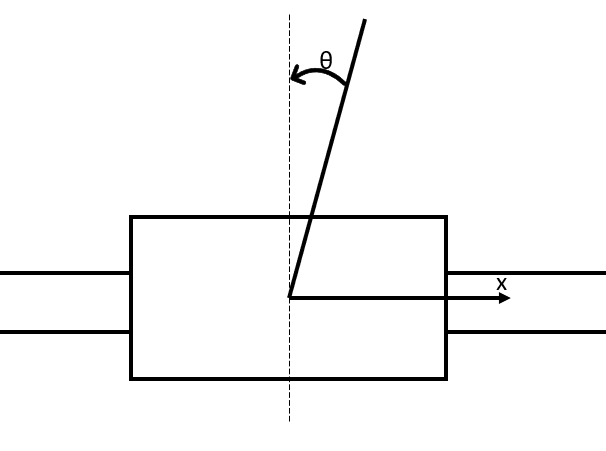
\includegraphics[width = 0.5\textwidth]{assets/figures/IllustrationPendule.svg.pdf}
  \caption{Illustration du pendule inversé demandé}
  \label{fig:Illustration}
\end{figure}

\section{Cas d'utilisation}\label{sec:CasUtil}
Lors des événements de la HEIG-VD, les visiteurs peuvent interagir avec la maquette de plusieurs manières. Une interface est présente et permet d'effectuer des opérations variées mais il est aussi possible de déstabiliser le pendule pour observer comment il arrive à se rattraper. Un affichage permettrait d'observer comment la régulation fonctionne en temps réel.
La figure \ref{fig:CasUtil} illustre ce cas d'utilisation typique.

\begin{figure}[H]
  \centering
  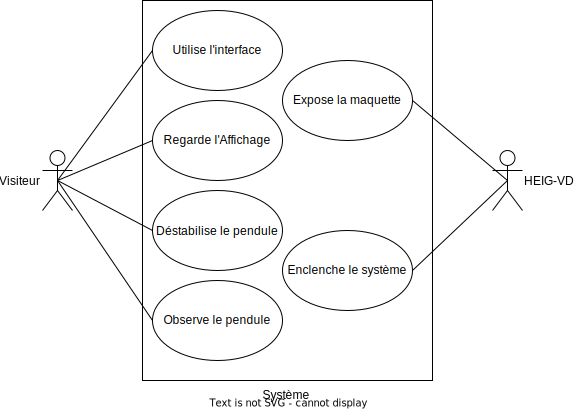
\includegraphics[width = 0.7\textwidth]{assets/figures/CasUtil.drawio.svg}
  \caption{Cas d'utilisation typique  du système à concevoir}
  \label{fig:CasUtil}
\end{figure}

\section{Analyse du besoin}\label{sec:AnalBesoins}
Suivant le cas d'utilisation illustré supra, les besoins identifiés de l'HEIG-VD sont exprimés au tableau \ref{tab:BesoinsHEIG}.

\begin{table}[H]
  \centering
  \caption{Besoins de l'HEIG-VD}
  \label{tab:BesoinsHEIG}
  \begin{tabular}{|l|l|}
    \hline
    \textbf{\#} & \textbf{Besoin}                                                   \\ \hline
    N1          & Intéresser de potentiels futurs   étudiants au métier d'ingénieur \\ \hline
    N2          & Disposer d'un système simple à   mettre en œuvre                  \\ \hline
    N3          & Assurer la sécurité des visiteurs   et des exposants              \\ \hline
    N4          & Présenter le domaine de la   régularisation numérique             \\ \hline
  \end{tabular}
\end{table}

Suivant le cas d'utilisation illustré supra, les besoins identifiés du visiteur sont exprimés au tableau \ref{tab:BesoinsVis}.

\begin{table}[H]
  \centering
  \caption{Besoins du visiteur}
  \label{tab:BesoinsVis}
  \begin{tabular}{|l|l|}
    \hline
    \textbf{\#} & \textbf{Besoin}                                    \\ \hline
    N5          & Se familiariser sur le sujet de la   régulation.   \\ \hline
    N6          & Se divertir à l'aide d'une   démonstration.        \\ \hline
    N7          & Découvrir le domaine des sciences   de l'ingénieur \\ \hline
  \end{tabular}
\end{table}

\section{Fonctions}\label{sec:Fonctions}
On détermine les fonctions suivantes dans le tableau \ref{tab:Fonctions} à partir des besoins de la HEIG-VD et des visiteurs qui sont indiqués dans le chapitre \ref{sec:AnalBesoins}, Analyse du besoin.

\begin{table}[H]
  \centering
  \caption{Fonctions du système à concevoir}
  \label{tab:Fonctions}
  \resizebox{\textwidth}{!}{%
    \begin{tabular}{|l|l|l|}
      \hline
      \textbf{\#} & \textbf{Fonctions système}                                                                     & \textbf{Besoin} \\ \hline
      F1          & Doit pouvoir tenir en équilibre                                                                & N5.1/N6.2       \\ \hline
      F2          & Doit pouvoir être autonome                                                                     & N5.1/N6.2       \\ \hline
      F3          & Doit pouvoir se mettre en équilibre tout seul depuis la position de repos                      & N5.1/N6.2       \\ \hline
      F4          & Doit permettre aux visiteurs d'effectuer des actions programmées sur le pendule.               & N5.1            \\ \hline
      F5          & Doit permettre aux visiteurs de déséquilibrer le système.                                      & N5.1            \\ \hline
      F6          & Doit expliquer aux visiteurs comment fonctionne le système.                                    & N5.1/N6.1       \\ \hline
      F7          & Doit pouvoir tenir sur une table.                                                              & N5.2            \\ \hline
      F8          & Doit pouvoir être alimenté facilement.                                                         & N5.2            \\ \hline
      F9          & Doit respecter les normes EN ISO 12100 de la SUVA \cite{NormeISO} sur la sécurité des machines & N5.3            \\ \hline
    \end{tabular}%
  }
\end{table}

Les fonctions sont disposées dans un diagramme FAST (c.f. Figure \ref{fig:AnalFAST}).

\begin{figure}[H]
  \centering
  \includegraphics[width = \textwidth]{assets/figures/AnalyseFAST.svg}
  \caption{Analyse FAST pour le pendule inversé}
  \label{fig:AnalFAST}
\end{figure}

\section{Exigences}\label{sec:Exigences}

\begin{table}[H]
  \centering
  \caption{Exigences de la solution retenue}
  \label{tab:Exigences}
  \resizebox{\textwidth}{!}{%
    \begin{tabular}{|l|l|l|l|}
      \hline
      \textbf{\#}                                                                                                             & \textbf{Exigence}                                                       & \textbf{Valeur attendue} & \textbf{Fonction} \\ \hline
      R1                                                                                                                      & Le système tient en équilibre tant qu'il est alimenté                   & Vrai                     & F7.1              \\ \hline
      R2                                                                                                                      & Le système retourne vers le centre lorsqu'il n'est pas perturbé         & Vrai                     & F7.2              \\ \hline
      R3                                                                                                                      &
      Le système est capable de se mettre en équilibre seul, à partir de sa position de repos                                 &
      Vrai                                                                                                                    &
      F7.3                                                                                                                                                                                                                                             \\ \hline
      R4                                                                                                                      & Temps d'amorçage de maximum 10 secondes                                 & \textless{}=10s          & F7.3              \\ \hline
      R5                                                                                                                      & Au moins 2 des 4 actions suivantes doivent être implémentées            & \textgreater{}=2         & F7.4              \\ \hline
      R6                                                                                                                      & Le pendule effectue un tour complet et reste équilibré                  & Vrai                     & F7.4              \\ \hline
      R7                                                                                                                      & Déplacement de bout en bout avec le pendule penché                      & Vrai                     & F7.4              \\ \hline
      R8                                                                                                                      & Le pendule s'arrête un moment et s'amorce d'un seul coup sec            & Vrai                     & F7.4              \\ \hline
      R9                                                                                                                      &
      Le chariot fait des mouvements de plus en plus amples pour rester en équilibre puis redevient graduellement plus stable &
      Vrai                                                                                                                    &
      F7.4                                                                                                                                                                                                                                             \\ \hline
      R10                                                                                                                     & Le système est capable de se rééquilibrer après une légère perturbation & Vrai                     & F7.5              \\ \hline
      R11                                                                                                                     &
      Les dimensions du système doivent rentrer dans un volume de 1400mm de largeur, 700mm de profondeur et 1000mm de hauteur &
      Vrai                                                                                                                    &
      F7.7                                                                                                                                                                                                                                             \\ \hline
      R12                                                                                                                     & Le système reste stable sur la table, même en fonctionnement            & Vrai                     & F7.7              \\ \hline
      R13                                                                                                                     & Le système peut être branché sur une prise 230V Suisse classique        & Vrai                     & F7.8              \\ \hline
      R14                                                                                                                     & Le système ne doit pas laisser la possibilité de se coincer les doigts  & Vrai                     & F7.9              \\ \hline
      R15                                                                                                                     & Le système possède un arrêt d'urgence                                   & Vrai                     & F7.9              \\ \hline
    \end{tabular}%
  }
\end{table}

\section{Etat de l'art}\label{sec:EtatArt}

\subsection{Segway}

L'exemple de pendule inversé le plus connu est le Segway \cite{Segway} qui utilise les perturbations des utilisateurs comme indications de la direction dans laquelle il est censé se diriger. Ainsi, en essayant de garder l'équilibre, il permet le déplacement de ses utilisateurs.

\begin{figure}[H]
  \centering
  \includegraphics[width = 0.3\textwidth]{assets/figures/Segway.png}
  \caption{Image d'un Segway \cite{Segway}}
  \label{fig:Segway}
\end{figure}

Ce genre de système n'est pas limité à un rail comme dans le projet courant. Ceci lui permet d'utiliser des roues pour effectuer le déplacement qui équilibre la personne.

\subsection{Pendule inversé}

Plusieurs projets de pendule inversé sont trouvables sur internet comme les deux suivants illustrés ci-dessous.
Le premier est un projet venant du site Instructables avec des éléments assez simples et peu chers visant à construire un pendule basique
pour introduire la régulation.

\begin{figure}[H]
  \centering
  \includegraphics[width = 0.8\textwidth]{assets/figures/PenduleInstructables.jpg}
  \caption{Image du montage du pendule inversé d'Instructables \cite{Instructables}}
  \label{fig:Instructables}
\end{figure}

On peut voir qu'une courroie est utilisée pour déplacer le chariot qui est guidé par des tubes en PVC et des roulements à billes. La mesure de l'angle, de la vitesse angulaire et de l'accélération angulaire du pendule se fait à l'aide d'un capteur d'inertie placé au bout de la tige.\\

Le pendule de l'entreprise Quanser est plus précis et possède une réponse plus rapide aux perturbations grâce au matériel plus coûteux utilisé pour le fabriquer. Il est aussi utilisé pour éduquer les utilisateurs sur la régulation bien qu'à un niveau plus avancé, spécifiquement dans un milieu universitaire.

\begin{figure}[H]
  \centering
  \includegraphics[width = 0.6\textwidth]{assets/figures/PenduleQuanser.png}
  \caption{Image du pendule inversé de Quanser \cite{Quanser}}
  \label{fig:Quanser}
\end{figure}

Celui-ci utilise deux encodeurs pour détecter la position angulaire de la tige et la position linéaire du pendule. Le système se déplace linéairement à l'aide d'un entrainement pignon/crémaillère et est guidé par une glissière.

\chapter{Calculs préliminaires}
Les calculs suivant sont nécessaires à la prise de décision pour les solutions.

\section{Valeurs utilisées}\label{sec:ValUtil}
Dans le tableau suivant se trouvent les valeurs constantes qui sont connues au préalable et qui seront utilisées dans les calculs.
La valeur d'accélération maximale voulue de 30~$m/s^2$ et une vitesse maximale de 5~m/s pour une course d'environ 1~m sont approximées.
Ces valeurs pourront être ajustées si jamais les calculs montrent qu'elles ne sont pas atteignables.

\begin{table}[H]
    \centering
    \caption{Valeurs utilisées pour les calculs}
    \label{tab:ValUtil}
    \begin{tabular}{|l|l|l|l|}
        \hline
        \textbf{Donnée}             & \textbf{Lettre} & \textbf{Valeur} & \textbf{Unité} \\ \hline
        Accélération max du chariot & a               & 30              & $m/s^2$        \\ \hline
        Vitesse max du chariot      & v               & 5               & $m/s$          \\ \hline
        Course du chariot           & l               & 1               & $m$            \\ \hline
    \end{tabular}%
\end{table}

La masse totale qui bouge est estimée à l'aide des approximations suivantes en prennant les éléments mentionnés dans le chapitre \ref{sec:PartMob}
et représentés dans la figure \ref{fig:StructPrelim}:
\begin{itemize}
    \item Tige en polycarbonate de 10~mm de diamètre: $\sim$50~g
    \item Glider moteur linéaire: $\sim$200~g
    \item Chariot du guidage linéaire: $\sim$100~g
    \item Resolver: $\sim$100~g
    \item Tête de lecture encodeur linéaire: $\sim$70~g
    \item Pièces créées en aluminium: $\sim$250-350~g
\end{itemize}

Il y aura donc une masse totale m en mouvement pouvant aller de 770 à 870~g. La valeur maximale sera utilisée pour déterminer la force maximale F
que le moteur doit appliquer pour atteindre l'accélération voulue en utilisant la formule suivante:

\begin{equation}\label{eq:ForceMot}
    F = m \cdot a = 0.87 \cdot 30 = 26.1~N
\end{equation}

Le moteur choisi devra appliquer une force d'au moins 26.1~N pour pouvoir obtenir l'accélération recherchée sur le pendule.\\

La course du moteur est aussi vérifiable afin d'être certain qu'elle soit suffisante pour atteindre la vitesse maximale du système. Il n'est possible
d'accélérer que sur la moitié de la course, car il faut décélérer sur la deuxième moitié afin d'éviter les impacts. Les formules suivantes sont
obtenues:

\begin{align}\label{eq:TempsMouv}
    \begin{split}
        x(t) = \frac{l}{2} = \frac{1}{2} \cdot a \cdot t^2 + v_0 \cdot t + x_0 \; avec \; v_0 = 0 \; et \; x_0 = 0 \\ \Rightarrow t = \sqrt{\frac{2 \cdot l}{2 \cdot a}} = \sqrt{\frac{2 \cdot 1}{2 \cdot 30}} = 183~ms
    \end{split}
\end{align}

\begin{equation}
    v(t) = a \cdot t + v_0 = 30 \cdot 0.183 + 0 = 5.48~m/s
\end{equation}

La valeur de vitesse maximale est bien atteignable avec cette course pour le chariot.

\chapter{Solutions}
\section{Description de la structure}\label{sec:DescStruct}
Avant de commencer à regarder les différentes solutions des points clés du projet il convient de se mettre d'accord
sur la structure principale où tout sera attaché. Cette dernière est faîte en profilé Item \cite{Item} comme convenu dans le decriptif
du projet. Le choix de profilé se portera sur le profilé 8 40x40 naturel. Afin de pouvoir le placer sur une table comme demandé, l'installation de pieds sera nécessaire. Les pieds proposé par Item ne
permettent pas une adhérence suffisante à la table et ne sont pas réglables. Elesa \cite{Elesa} possède une grande variété de pieds ce qui
a permis de trouver exactement ce qui était recherché pour ce projet. La fabrication d'une pièce (plan dans les Annexes) pour pouvoir attacher
les pieds au reste de la structure est donc nécessaire. Cette dernière aura un perçage taraudé M10 pour visser un pieds et un lamage M8 pour
une vis six pans creux à tête cylindrique qui se fixe sur le côté taraudé des profilés. Voici à quoi ressemble la pièce en question.

\begin{figure}[H]
  \centering
  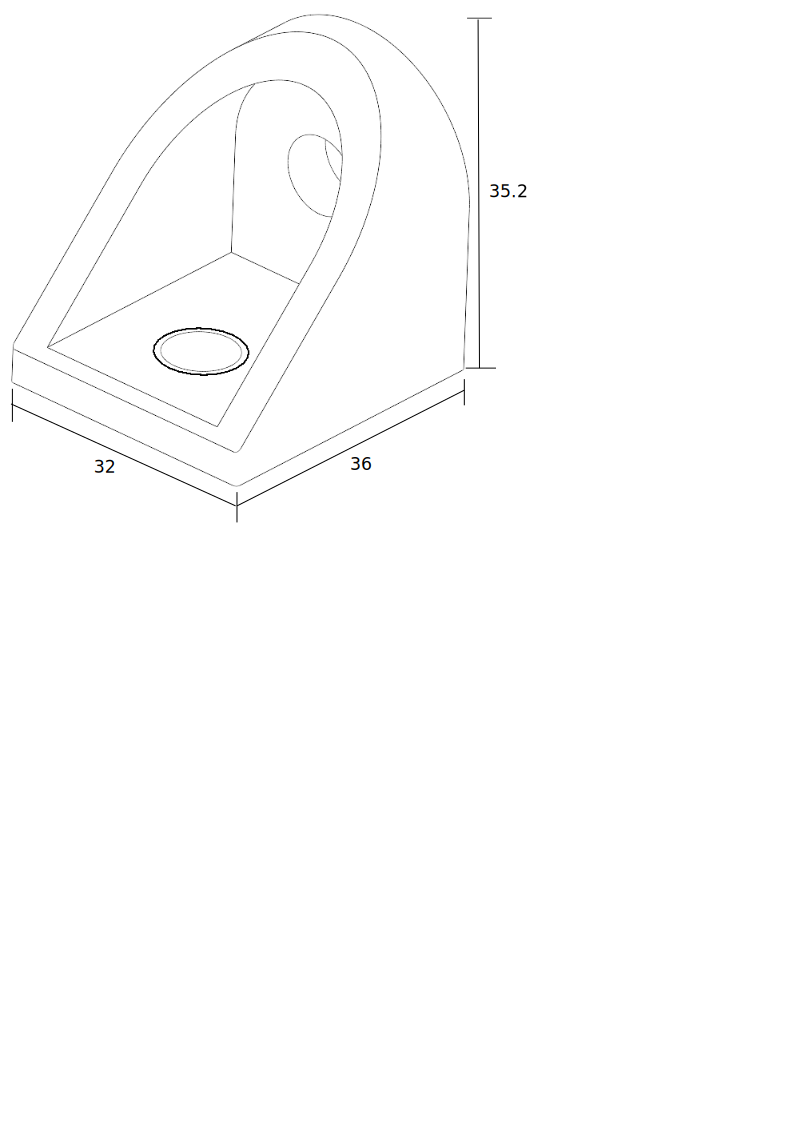
\includegraphics[width = 0.4\textwidth]{assets/figures/SupportPieds.png}
  \caption{Représentation du support pour les pieds du système}
  \label{fig:SupPieds}
\end{figure}

La structure complète avec les pieds et ses supports ressemble à ceci.
\begin{figure}[H]
  \centering
  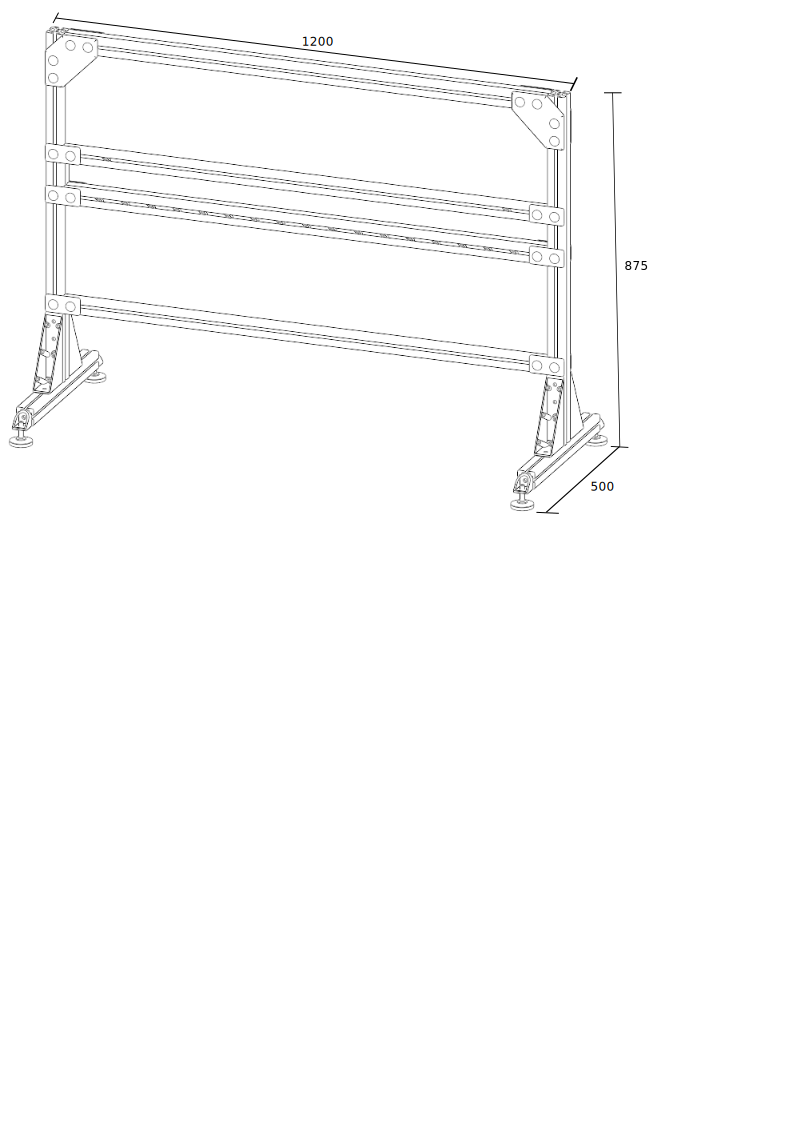
\includegraphics[width = 0.8\textwidth]{assets/figures/Structure.png}
  \caption{Représentation de la structure en 3D}
  \label{fig:DescStruct}
\end{figure}

On peut voir que la structure utilise quatre grands profilés horizontaux, deux aux extrémités et deux au centre. Ce sera sur les deux profilés du centre que
les éléments du pendule pourront venir se fixer plus tard. Deux plaques sont mises entre des profilés pour à la fois rendre le projet présentable
en cachant les éléments arrière et à la fois rendre la structure plus rigide.

\section{Catalogue de solutions}\label{sec:CatSol}
Maintenant que la structure est connue, il est possible d'étudier les différentes solutions sur les points clés du projet.
Les points principaux sont: le moteur linéaire, le guidage et la mesure de position linéaire.

\subsection{Moteur linéaire}
\subsubsection{A: Commander un moteur linéaire}
Les offres suivantes ont été faites par des entreprises contactées lors de ce travail.

\begin{table}[H]
  \centering
  \caption{Offres pour le moteur linéaire}
  \label{tab:OffreMot}
  \resizebox{\textwidth}{!}{%
    \begin{tabular}{|l|l|l|l|l|}
      \hline
      Entreprise                                         & Prix                       & Délai de livraison              & Poids chariot          & Force continue \\ \hline
      DD auto Tech \cite{DDautoTech}                     & 1105 CHF                   & \cellcolor{red}16 semaines      & 60g                    & 39N            \\ \hline
      ESR Pollmeier \cite{ESRPollmeier}                  & \cellcolor{red}-           & \cellcolor{red}16 semaines      & \cellcolor{yellow}600g & 29N            \\ \hline
      TDS Precision Products \cite{TDSPrecisionProducts} & 1020 CHF                   & \cellcolor{yellow}8-10 semaines & 180g                   & 26.4N          \\ \hline
      Heidenhain \cite{Heidenhain}/Etel \cite{Etel}      & \cellcolor{yellow}3000 CHF & 7 semaines                      & 100g                   & 31.9N          \\ \hline
    \end{tabular}%
  }
\end{table}

L'offre la plus intéressante est celle de TDS Precision avec un prix raisonnable et un temps de livraison un peu plus long mais qui rentre dans le planning.

\subsubsection{B: Utiliser un rail magnétique déjà en stock}
Un rail magnétique Etel de 1024mm de longueur est en stock à la HEIG et nécessiterait uniquement la commande de la partie mobile. Cependant ce
rail est plus lourd et encombrant que certaines des solutions commandables. Cela reste un bon plan de secours en cas de problème d'approvisionnement.

\subsection{Guidage linéaire}
\subsubsection{A: Commander un guidage linéaire avec mesure de position intégré}
Les offres suivantes ont été faites par des entreprises contactées lors de ce travail.

\begin{table}[H]
  \centering
  \caption{Offres pour le guidage linéaire avec mesure de position}
  \label{tab:OffreGuidPos}
  \resizebox{\textwidth}{!}{%
    \begin{tabular}{|l|l|l|l|l|}
      \hline
      Entreprise                       & Prix                             & Délai de livraison & Longueur & Poids chariot                \\ \hline
      Schneeberger \cite{Schneeberger} & \cellcolor[HTML]{FF0000}1369 CHF & 4 semaines         & 995mm    & 84g                          \\ \hline
      Hiwin \cite{Hiwin}               & \cellcolor[HTML]{FF0000}1171 CHF & 3 semaines         & 1100mm   & \cellcolor[HTML]{FF0000}420g \\ \hline
    \end{tabular}%
  }
\end{table}

L'offre la plus intéressante est celle de Schneeberger avec un chariot beaucoup plus léger, cependant le prix est trop élevé pour pouvoir considérer cette solution.

\subsubsection{B: Commander guidage linéaire et le capteur de position séparément}
\textbf{ - Capteur:}
\newline
Les offres suivantes ont été faites par des entreprises contactées lors de ce travail.

\begin{table}[H]
  \centering
  \caption{Offres pour le capteur pour la mesure de position}
  \label{tab:OffrePos}
  \resizebox{\textwidth}{!}{%
    \begin{tabular}{|l|l|l|l|l|}
      \hline
      Entreprise                   & Prix                             & Délai de livraison                  & Longueur                       & Poids tête                  \\ \hline
      RLS \cite{RLS}               & \cellcolor[HTML]{FFFFFF}640 CHF  & \cellcolor[HTML]{FFFFFF}4 semaines  & \cellcolor[HTML]{FFFFFF}1000mm & 32g                         \\ \hline
      Heidenhain \cite{Heidenhain} & \cellcolor[HTML]{FFFF00}1080 CHF & \cellcolor[HTML]{FF0000}16 semaines & \cellcolor[HTML]{FFFFFF}1040mm & \cellcolor[HTML]{FFFFFF}20g \\ \hline
    \end{tabular}%
  }
\end{table}

\textbf{ - Guidage:}
\newline
Les offres suivantes ont été faites par des entreprises contactées lors de ce travail.

\begin{table}[H]
  \centering
  \caption{Offres pour le guidage}
  \label{tab:OffreGuid1}
  \resizebox{\textwidth}{!}{%
    \begin{tabular}{|l|l|l|l|l|}
      \hline
      Entreprise             & Prix             & Délai de livraison & Longueur & Poids chariot                \\ \hline
      Ewellix \cite{Ewellix} & \cellcolor{red}- & \cellcolor{red}-   & 995mm    & \cellcolor[HTML]{FF0000}400g \\ \hline
      Rollon \cite{Rollon}   & \cellcolor{red}- & \cellcolor{red}-   & 1000mm   & 170g                         \\ \hline
      Igus \cite{Igus}       & 130 CHF          & 10 jours           & 1100mm   & \cellcolor[HTML]{FFFF00}260g \\ \hline
      Igus \cite{Igus}       & 150 CHF          & 2 jours            & 1100mm   & \cellcolor[HTML]{FFFFFF}110g \\ \hline
    \end{tabular}%
  }
\end{table}

Les deux offres choisies sont donc la règle linéaire de RLS et le second rail linéaire de Igus. Le poids minime du chariot Igus est un avantage considérable
et le temps de livraison plus court chez RLS sont les facteurs clés de ce choix.

\subsubsection{C: Commander guidage linéaire et utiliser un capteur déjà en stock}
\textbf{ - Capteur:}
\newline
Le capteur en stock est une règle linéaire LIDA 405 de 840mm de plage mesurable avec la tête de lecture et fixation. La seule partie à commander
est le support pour le ruban. Cette solution nécessite un temps de livraison inférieur à ceux des capteurs commandables et coute beaucoup moins cher.

\textbf{ - Guidage:}
\newline

\begin{table}[H]
  \centering
  \caption{Offres pour le guidage}
  \label{tab:OffreGuid2}
  \resizebox{\textwidth}{!}{%
    \begin{tabular}{|l|l|l|l|l|}
      \hline
      Entreprise             & Prix             & Délai de livraison & Longueur & Poids chariot                \\ \hline
      Ewellix \cite{Ewellix} & \cellcolor{red}- & \cellcolor{red}-   & 995mm    & \cellcolor[HTML]{FF0000}400g \\ \hline
      Rollon \cite{Rollon}   & \cellcolor{red}- & \cellcolor{red}-   & 1000mm   & 170g                         \\ \hline
      Igus \cite{Igus}       & 130 CHF          & 10 jours           & 1100mm   & \cellcolor[HTML]{FFFF00}260g \\ \hline
      Igus \cite{Igus}       & 150 CHF          & 2 jours            & 1100mm   & \cellcolor[HTML]{FFFFFF}110g \\ \hline
    \end{tabular}%
  }
\end{table}

Cette solution utilisera la règle linéaire de chez Heidenhain en stock et le second rail Igus grâce au poids minime de son chariot.

\section{Solutions choisies}\label{sec:SolChoix}

La solution choisie pour le moteur linéaire est la solution A, c'est à dire la commande d'un nouveau moteur chez TDS Precision \cite{TDSPrecisionProducts}. Ce dernier
sera fixé à l'arrière de la structure sur un des profilé du centre.\\

La solution choisie pour le guidage linéaire est la solution C, c'est à dire la commande d'un guidage linéaire chez Igus \cite{Igus} et l'utilisation d'une
règle linéaire de chez Heidenhain \cite{Heidenhain} appartenant déjà à la HEIG. Le rail peut être fixé sur la partie avant des profilés et la règle linéaire peut
être placée sur la partie arrière du deuxième profilé. La datasheet de ces composants se trouvent dans les Annexes de ce document. Le résultat du placement de ces
éléments peut être observé sur les figures suivante.

\begin{figure}[H]
  \centering
  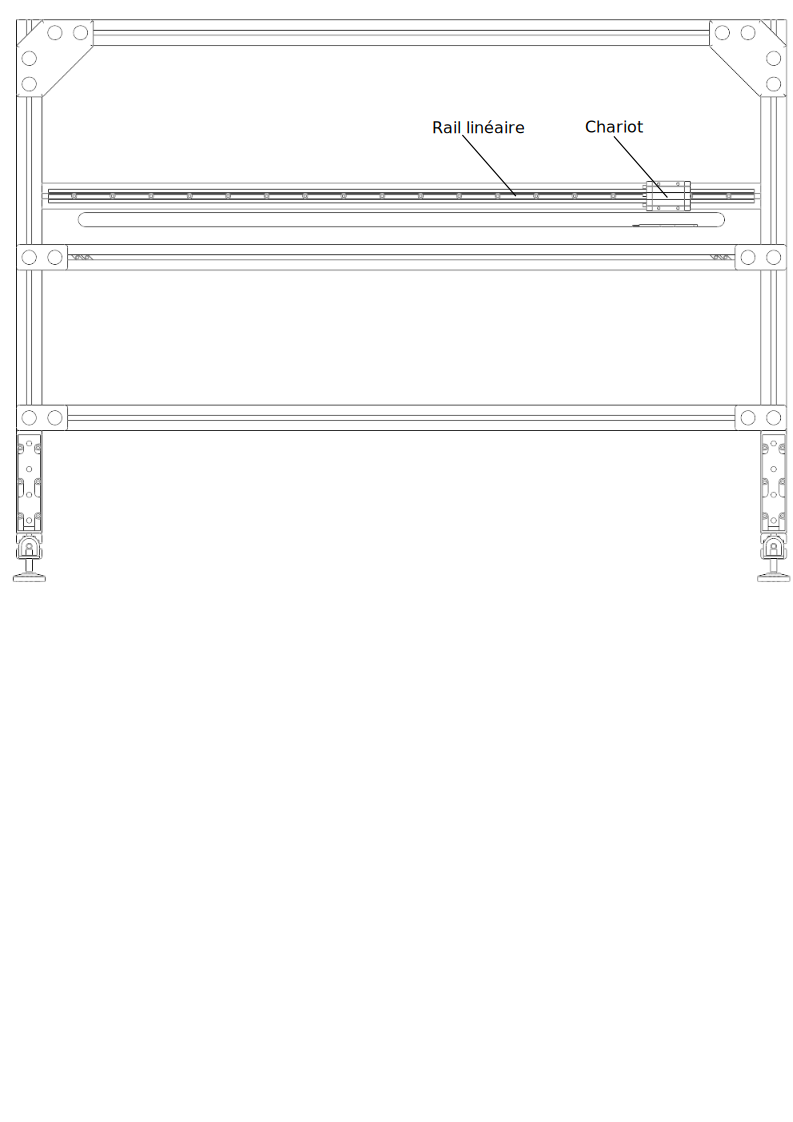
\includegraphics[width = \textwidth]{assets/figures/VueFace.png}
  \caption{Représentation de la structure en 3D de face avec l'ajout des éléments des solutions}
  \label{fig:VueFace}
\end{figure}

\begin{figure}[H]
  \centering
  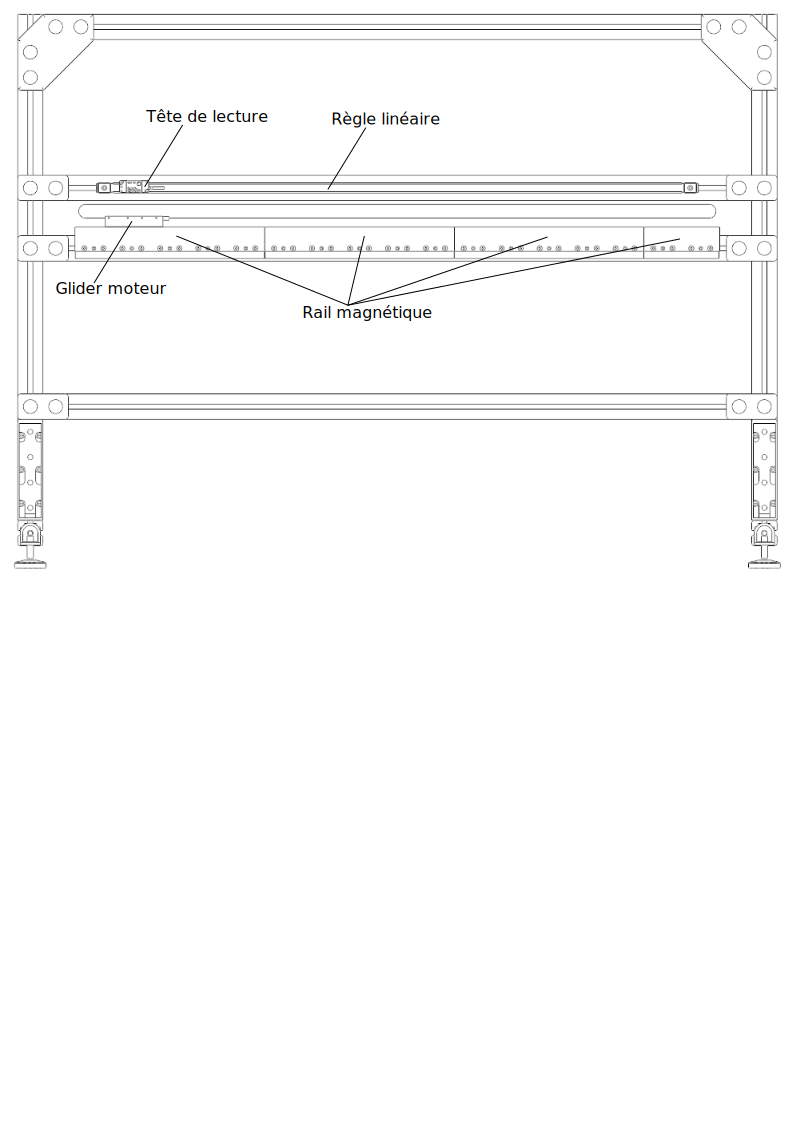
\includegraphics[width = \textwidth]{assets/figures/VueDerriere.png}
  \caption{Représentation de la structure en 3D de derrière avec l'ajout des éléments des solutions}
  \label{fig:VueDerriere}
\end{figure}

Maintenant que les éléments sont en place, il faut les lier ensemble avec des pièces faîtes sur mesure. Toutes les pièces sont faîtes
d'aluminium EN-AW 6082. la liaison entre le chariot du guidage et le glider du moteur va se faire en deux pièces vissées ensemble. La pièce
connectée au chariot devra accueilir deux roulements qui servent à fair tourner la partie qui tient la tige du pendule. Une zone pour placer
un anneau de LEDs est aussi nécessaire afin de pouvoir illuminer la tige. Enfin, cette pièce devra aussi accueilir l'encodeur pour la position
angulaire. La fixation sur le chariot se fait avec quatre vis M5 ce qui nécessitera donc des lamages. La fixation sur l'autre pièce se fait sur
le dessous de la pièce avec quatres taraudages M5. Un rebord pour l'indexage avec l'autre pièce est aussi présent. On obtient la pièce suivante.

\begin{figure}[H]
  \centering
  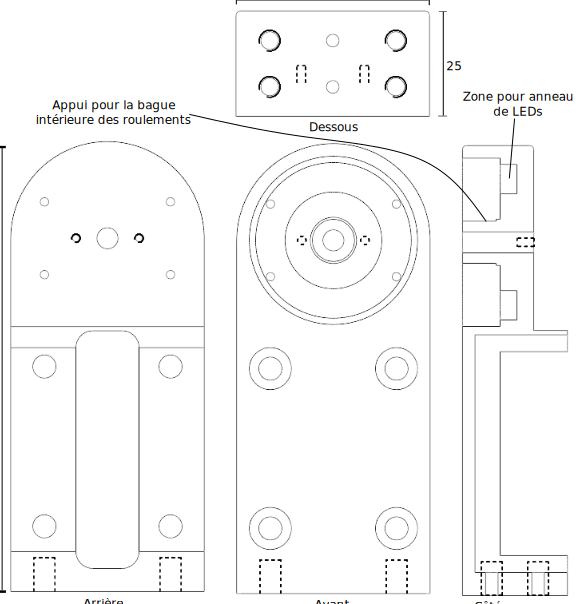
\includegraphics[width = 0.4\textwidth]{assets/figures/LiaisonChariot.png}
  \caption{Représentation de la pièce de liaison du chariot}
  \label{fig:LiaisonChariot}
\end{figure}

La seconde pièce devra évidemment se lier avec la première mais aussi avec le moteur. La première pièce ayant les taraudages, celle-ci aura quatre
lamages M5. Pour la fixation au moteur, quatre lamages M3 suffiront. Deux autres éléments viennent encore se fixer sur cette pièce: le support de
la tête de lecture pour la règle linéaire et la chaine porte câble. Pour le support de tête de lecture, trois taraudages M4 sont placés sur un côté
alors que deux trous taraudés sont utilisés pour fixer la chaine porte câble. Finalement, voilà à quoi ressemble la pièce.

\begin{figure}[H]
  \centering
  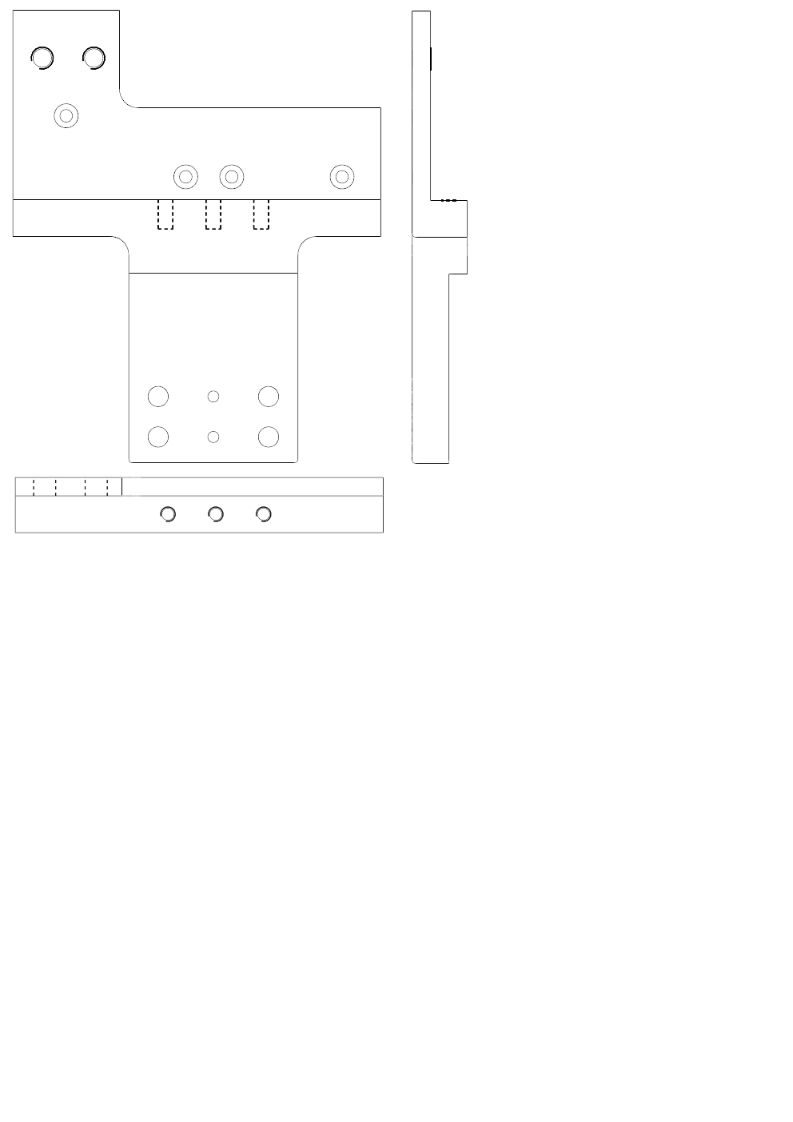
\includegraphics[width = 0.4\textwidth]{assets/figures/LiaisonMoteur.png}
  \caption{Représentation de la pièce de liaison du moteur}
  \label{fig:LiaisonMoteur}
\end{figure}

\chapter{Mécanique}
Plusieurs pièces mécaniques ont dû être développées pendant ce projet comme par exemple le support de pieds  qui a déjà été décrit au chapitre \ref{sec:DescStruct}.
Maintenant que les éléments sont en place, il faut les lier ensemble avec des pièces faites sur mesure. Toutes les pièces sont faîtes
d'aluminium EN-AW 6082 sauf si mentionné autrement.

\section{Liaison Moteur-Glider}\label{sec:LiaisonMotGlid}
La liaison entre le chariot du guidage et le \gls{glider} du moteur va se faire en deux pièces vissées ensemble. La pièce
connectée au chariot devra accueillir deux roulements qui servent à faire tourner la partie qui tient la tige du pendule. Une zone pour placer
un anneau de LEDs est aussi nécessaire afin de pouvoir illuminer la tige. Enfin, cette pièce devra aussi accueillir l'encodeur pour la position
angulaire. La fixation sur le chariot se fait avec quatre vis M5 ce qui nécessitera donc des lamages. La fixation sur l'autre pièce se fait sur
le dessous de la pièce avec quatre taraudages M5. Un rebord pour l'indexage avec l'autre pièce est aussi présent. On obtient la pièce suivante.

\begin{figure}[H]
  \centering
  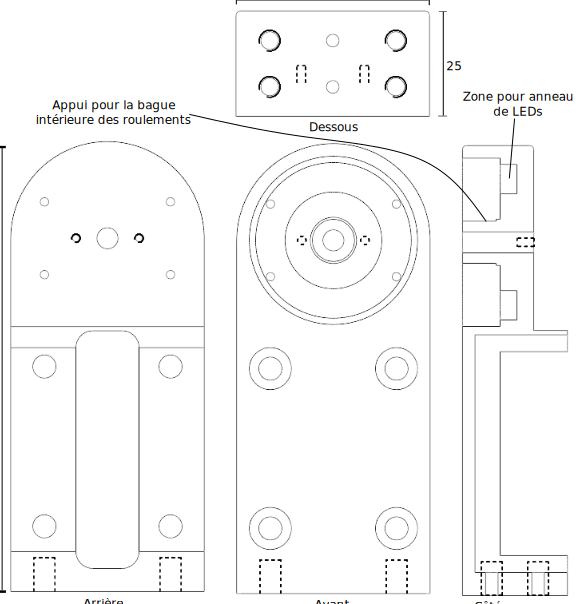
\includegraphics[width = 0.4\textwidth]{assets/figures/LiaisonChariot.png}
  \caption{Représentation de la pièce de liaison du chariot}
  \label{fig:LiaisonChariot}
\end{figure}

La seconde pièce devra évidemment se lier avec la première, mais aussi avec le moteur. La première pièce ayant les taraudages, celle-ci aura quatre
lamages M5. Pour la fixation au moteur, quatre lamages M3 suffiront. Deux autres éléments viennent encore se fixer sur cette pièce: le support de
la tête de lecture pour la règle linéaire et la chaîne porte-câbles. Pour le support de tête de lecture, trois taraudages M4 sont placés sur un côté,
alors que deux trous taraudés sont utilisés pour fixer la chaîne porte-câbles. Finalement, voilà à quoi ressemble la pièce.

\begin{figure}[H]
  \centering
  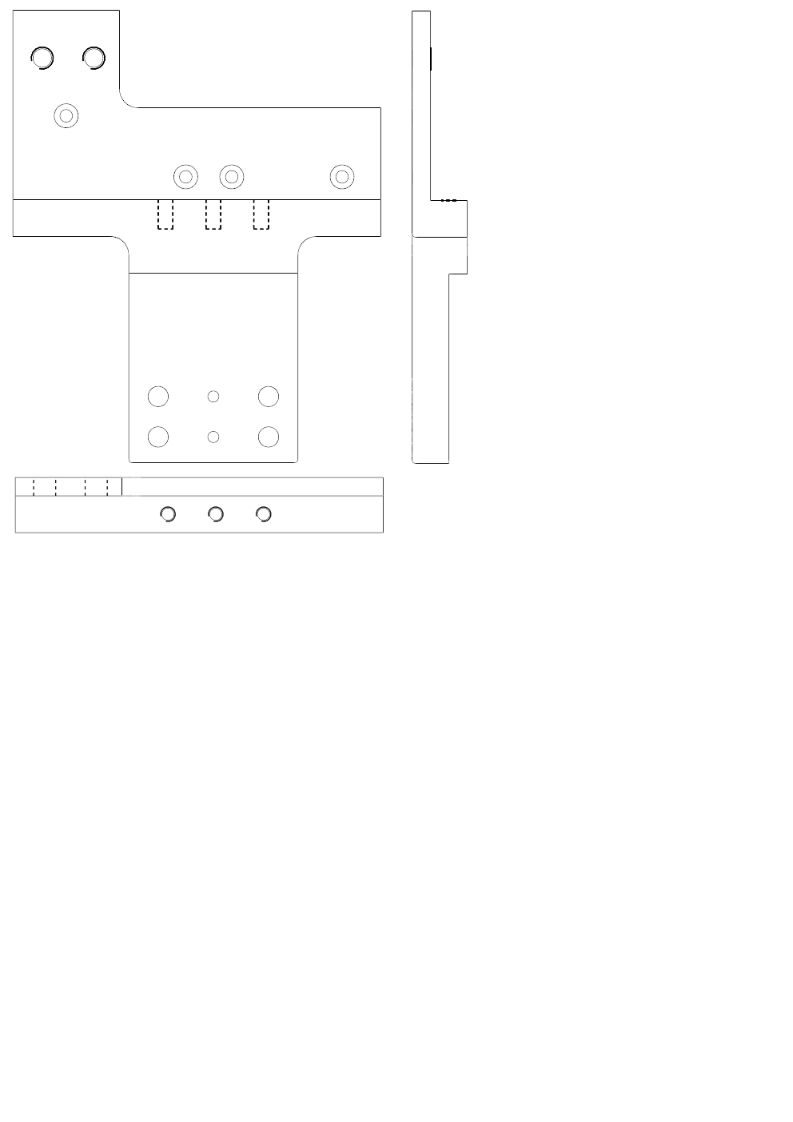
\includegraphics[width = 0.4\textwidth]{assets/figures/LiaisonMoteur.png}
  \caption{Représentation de la pièce de liaison du moteur}
  \label{fig:LiaisonMoteur}
\end{figure}

L'assemblage de ces pièces entre elles et avec leur liaisons directes donne la représentation suivante.

\begin{figure}[H]
  \centering
  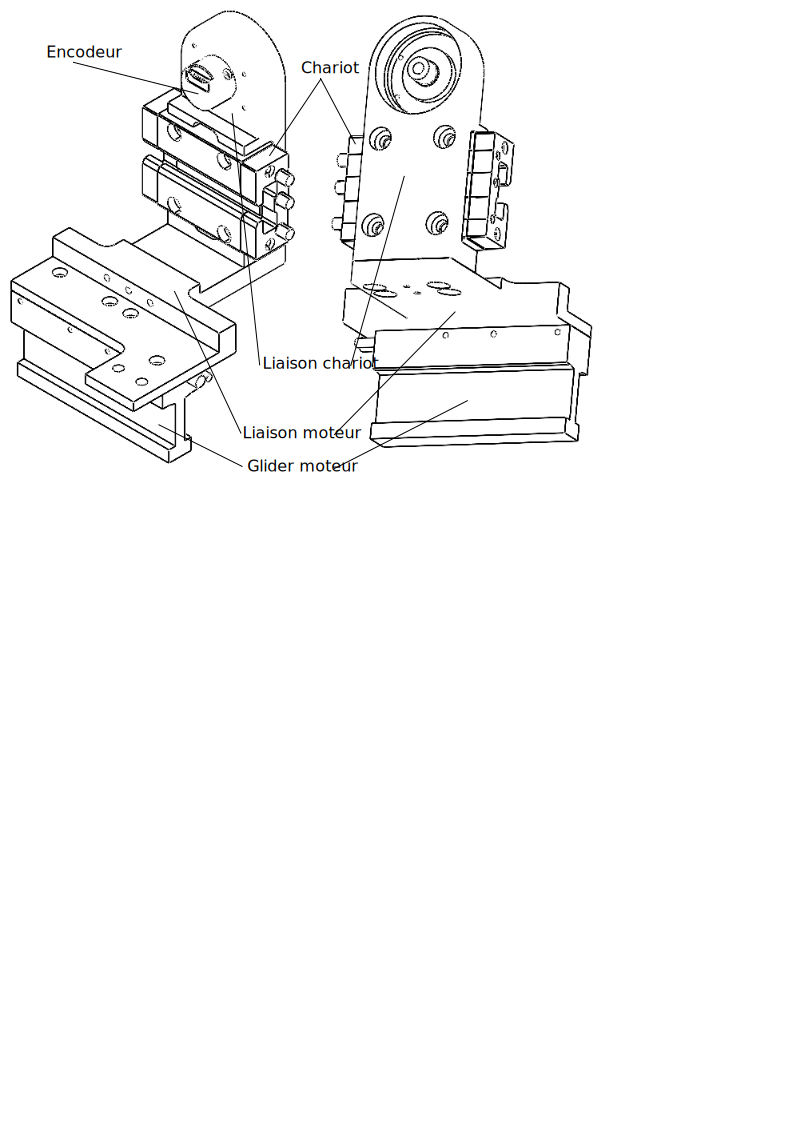
\includegraphics[width = 0.8\textwidth]{assets/figures/AssemblageGuidageEntrainement.png}
  \caption{Représentation de l'assemblage des pièces de guidage et d'entrainement du système}
  \label{fig:AssGuiEntr}
\end{figure}

\section{Support tête de lecture}\label{sec:SupTeteLect}
Le support de la tête de lecture de la règle linéaire est fixé sur la pièce attachée au moteur comme mentionné plus haut. Elle aura donc trois
lamages M4 pour se fixer à la liaison moteur et aussi deux trous de passage pour vis M3 pour la tête de lecture. Un trou supplémentaire est ajouté
pour faire le réglage en position de la tête. La pièce obtenue est la suivante.

\begin{figure}[H]
  \centering
  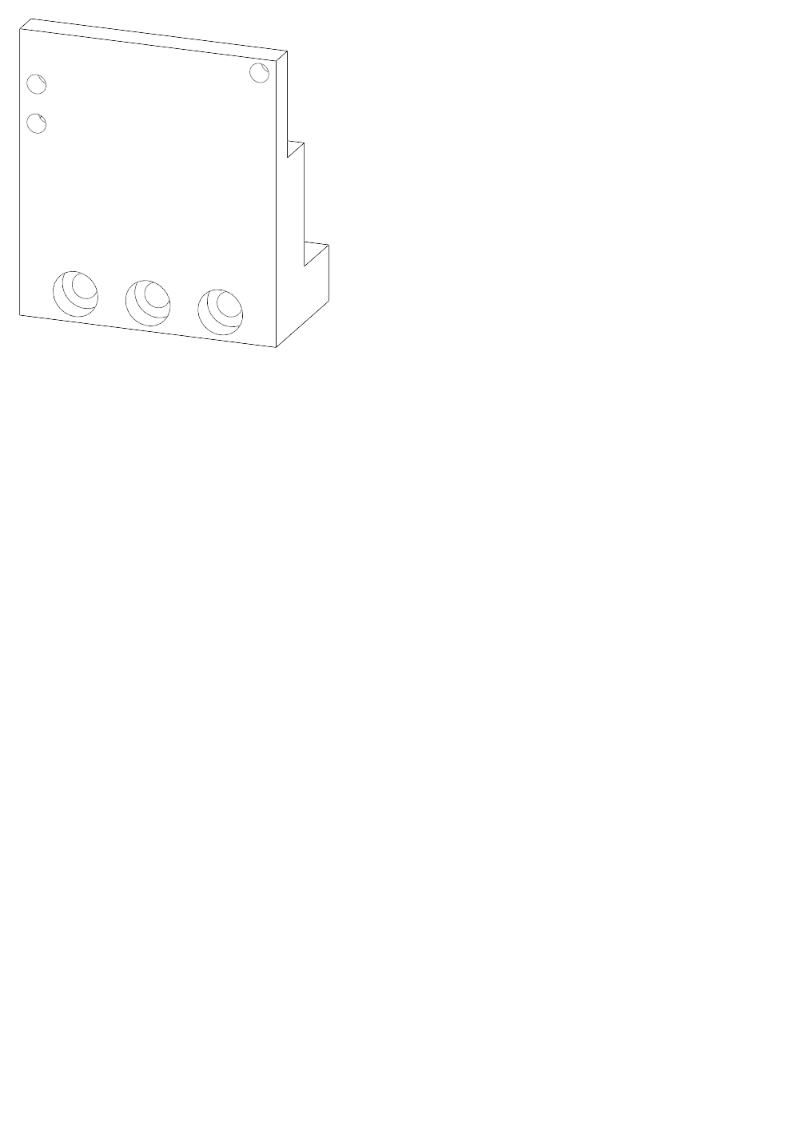
\includegraphics[width = 0.4\textwidth]{assets/figures/SupportTeteLecture.png}
  \caption{Représentation du support de tête de lecture}
  \label{fig:SupTeteLect}
\end{figure}

Voici une représentation avec le support monté sur la liaison au moteur et avec la tête de lecture.

\begin{figure}[H]
  \centering
  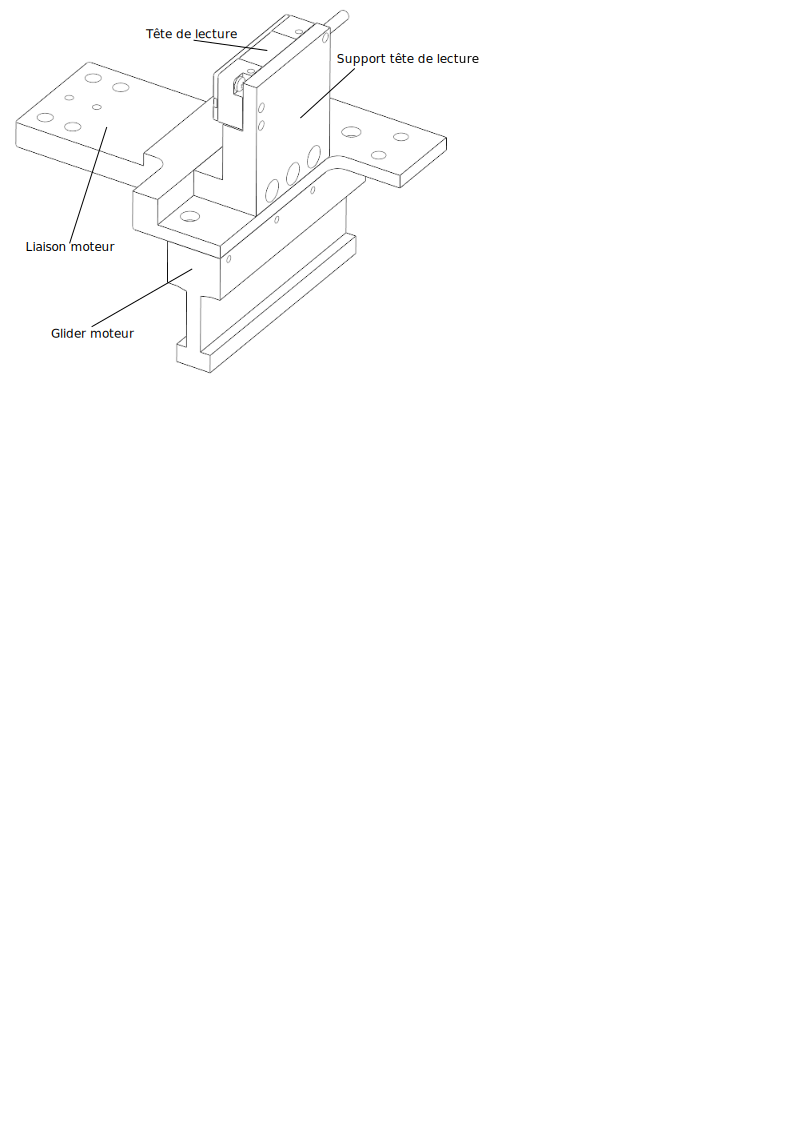
\includegraphics[width = 0.6\textwidth]{assets/figures/AssemblageMesureLineaire.png}
  \caption{Représentation du support de tête de lecture assemblée avec les pièces proches dans le système}
  \label{fig:AssMesLin}
\end{figure}

\section{Support fin de course}\label{sec:SupFinCourse}
Les capteurs de fins de course seront placés à l'arrière de la structure de chaque côté du système. Ces capteurs se fixent dans des rainures et
il faut un petit support pour pouvoir tenir le capteur et l'accrocher au système avec une vis d'où le lamage M3 nécessaire. Dans ce cas-ci, le support ne subit pas d'effort particulier
ce qui veut dire qu'il peut être fait en \acrshort{PLA} par impression 3D. Voici à quoi ressemble cette pièce.

\begin{figure}[H]
  \centering
  \includegraphics[width = 0.4\textwidth]{assets/figures/SupportFinCourse.png}
  \caption{Représentation du support de fin de course}
  \label{fig:SupFinCourse}
\end{figure}

\section{Support amortisseur}\label{sec:SupAmort}
Les amortisseurs se trouvent à l'avant du système au bout de chaque côté de la course. Leur support doit être assez épais pour pouvoir supporter
les chocs. Un trou taraudé M10 est nécessaire pour fixer l'amortisseur et deux lamages M4 permettent la fixation sur le profilé. Les deux amortisseurs
étant dans des directions opposées, il faut créer un deux support symétriques pour pouvoir les fixer. Voici l'image d'un des supports.

\begin{figure}[H]
  \centering
  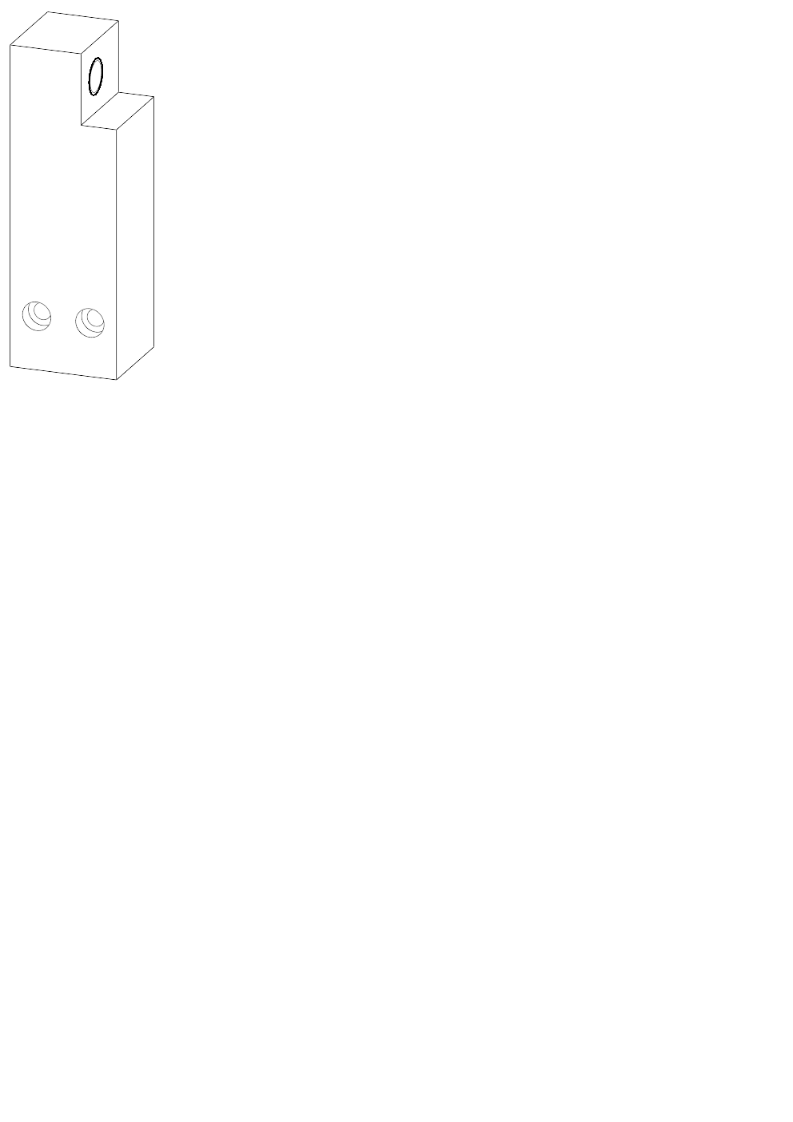
\includegraphics[width = 0.3\textwidth]{assets/figures/SupportAmortisseur.png}
  \caption{Représentation du support de l'amortisseur}
  \label{fig:SupAmort}
\end{figure}

Le placement des supports de l'amortisseur et du fin de course sur un des côtés est visible sur cette image.

\begin{figure}[H]
  \centering
  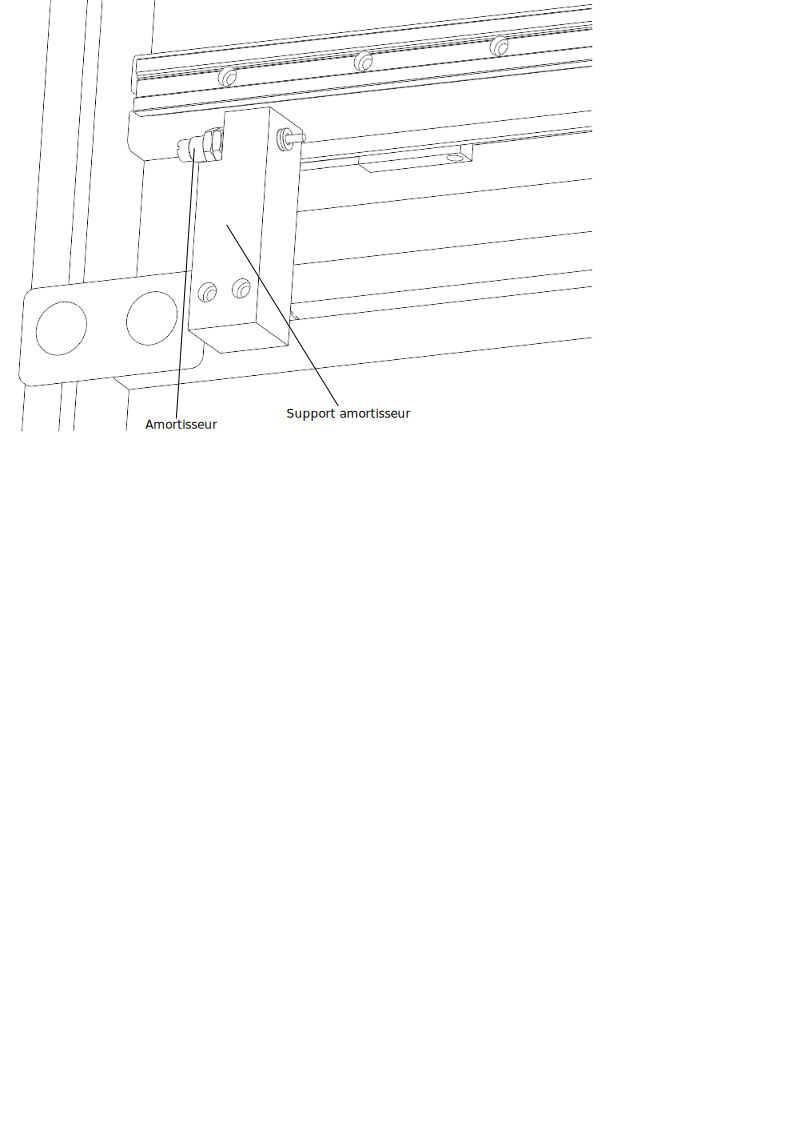
\includegraphics[width = 0.8\textwidth]{assets/figures/PlacementSupports.png}
  \caption{Représentation du placement des supports de fin de course et de l'amortisseur pour un côté}
  \label{fig:PlaceSup}
\end{figure}

\section{Partie tournante}\label{sec:PartieTour}
La partie tournante du système est composée de plusieurs pièces, dont une en \acrshort{PC}. Tout d'abord, la partie en contact direct
avec les roulements et en couplage avec l'encodeur. Cette partie est aussi attachée à une autre pièce, le couplage à la tige, à l'aide de
quatre taraudages M2. Voici à quoi elle ressemble.

\begin{figure}[H]
  \centering
  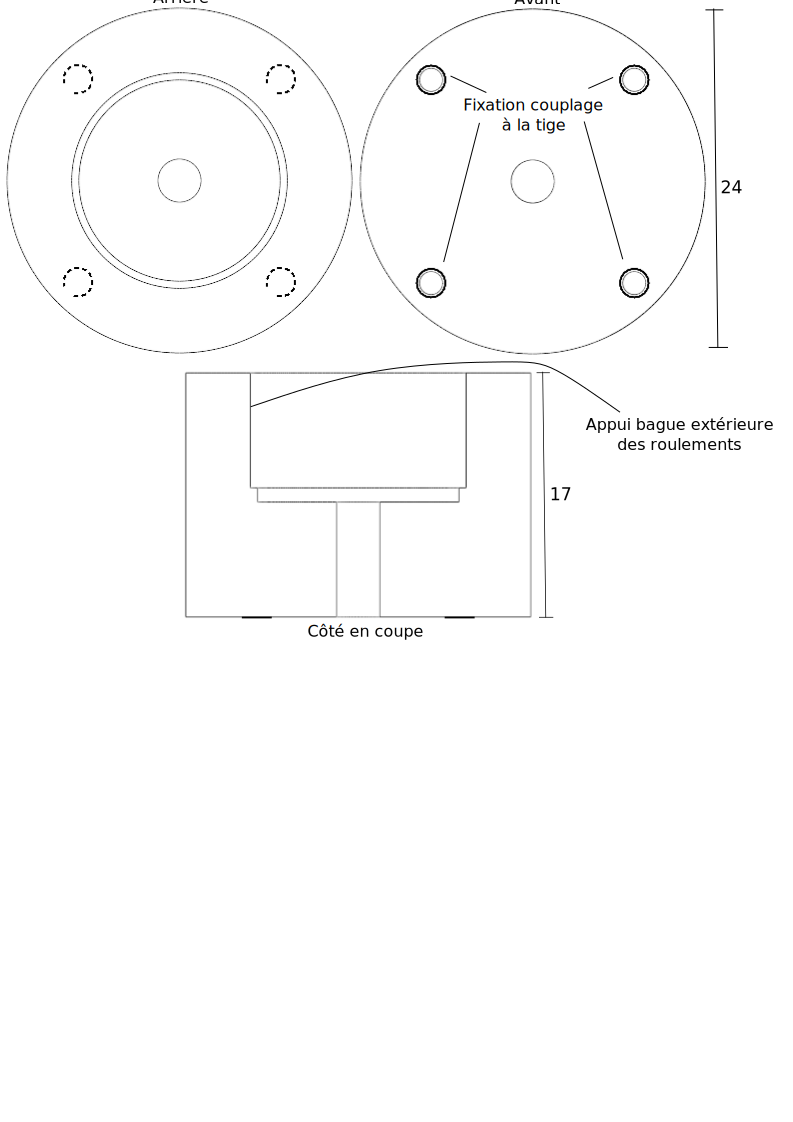
\includegraphics[width = 0.9\textwidth]{assets/figures/CouplageEncodeur.png}
  \caption{Représentation du couplage à l'encodeur}
  \label{fig:CouplEnco}
\end{figure}

La pièce de couplage à la tige qui est attachée à celle montrée sur la figure \ref{fig:CouplEnco} est en \acrshort{PC}. Elle possède donc quatre
lamages M2 pour pouvoir se visser sur la pièce précédente et aussi un perçage de 10~mm de diamètre pour venir fixer la tige par serrage.
La pièce ressemble à ceci.

\begin{figure}[H]
  \centering
  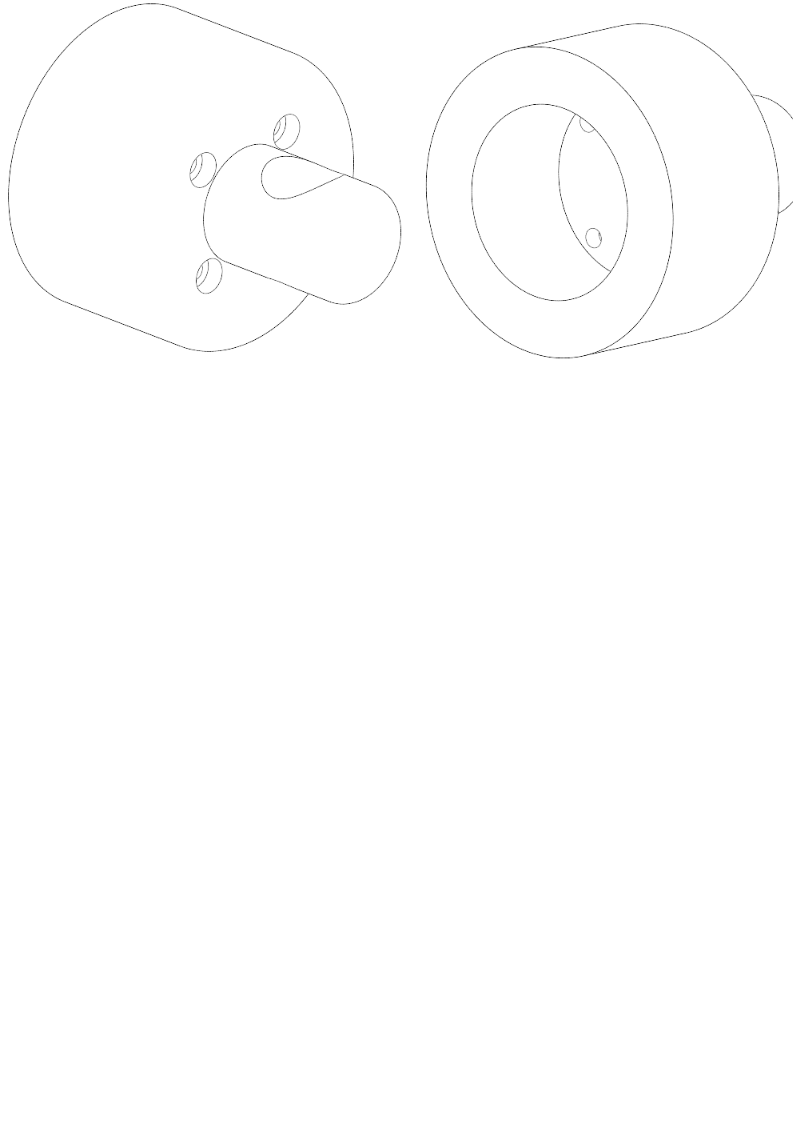
\includegraphics[width = 0.9\textwidth]{assets/figures/CouplageTige.png}
  \caption{Représentation du couplage à la tige}
  \label{fig:CouplTige}
\end{figure}

Il y a aussi la tige, elle aussi en \acrshort{PC}, qui vient se placer dans le perçage de 10~mm de la pièce précédente. La tige a donc un
diamètre lui aussi égal à 10~mm et une longueur de 420~mm. Aucune autre modification n'est apportée à la tige à part un chanfrein afin d'éviter
les arêtes coupantes.\\

L'assemblage de ces différentes pièces ainsi que de la liaison au chariot et l'encodeur donne la représentation suivante.

\begin{figure}[H]
  \centering
  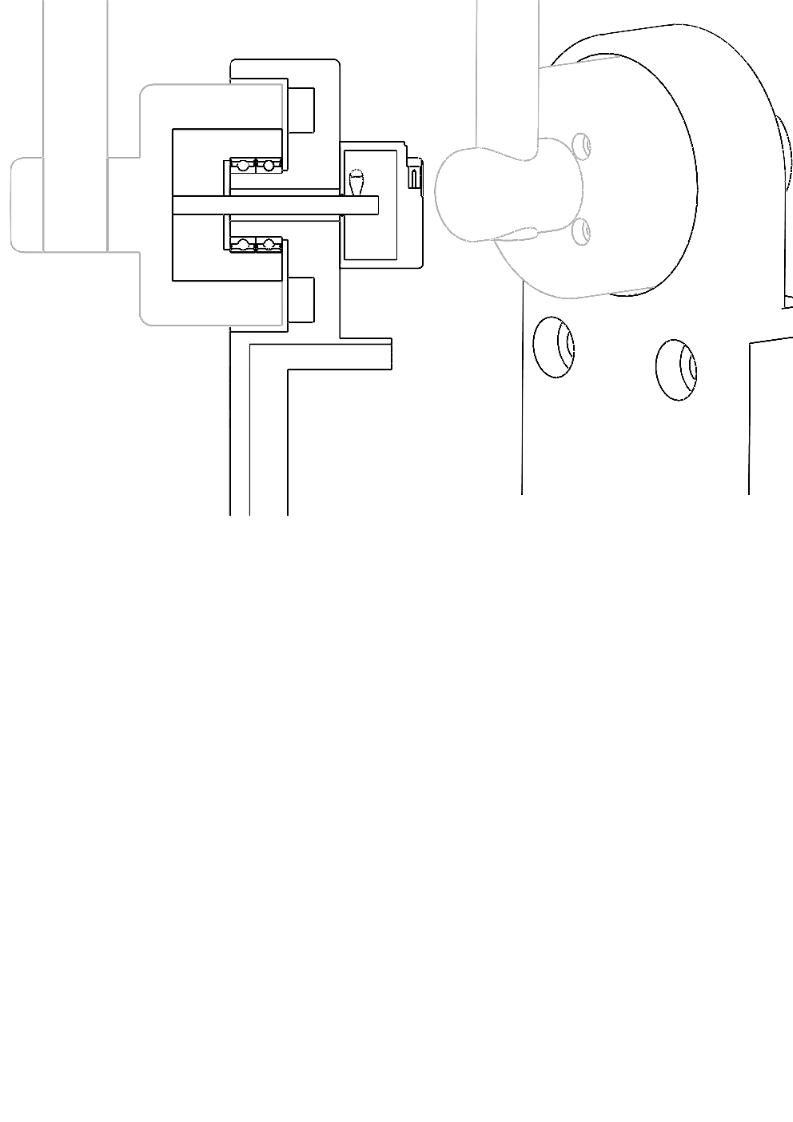
\includegraphics[width = 0.7\textwidth]{assets/figures/AssemblagePartieTournante.png}
  \caption{Représentation de l'assemblage des parties tournantes et leurs connections directes}
  \label{fig:AssPartieTour}
\end{figure}


\section{Support pour chaîne porte-câbles}\label{sec:SupChainCable}
La chaîne porte-câbles est fixée d'un côté à la liaison moteur comme précisé plus haut au chapitre \ref{sec:LiaisonMotGlid}. L'autre côté est
attaché au support pour chaîne porte-câbles qui est lui-même fixé sur un profilé. Deux passages de vis M4 sont présents pour la fixation sur
le profilé ainsi que deux autres passages de vis M6 pour la fixation de la chaîne. Il y a aussi un dégagement de matière afin de pouvoir faire
passer les câbles qui sortent de la chaîne et qui continuent plus bas vers le boîtier électrique. Cette pièce est fabriquée en tôle pliée et
nécessite un alliage d'aluminium différent, l'aluminium EN-AW 5052. Voici une image du support pour la chaîne.

\begin{figure}[H]
  \centering
  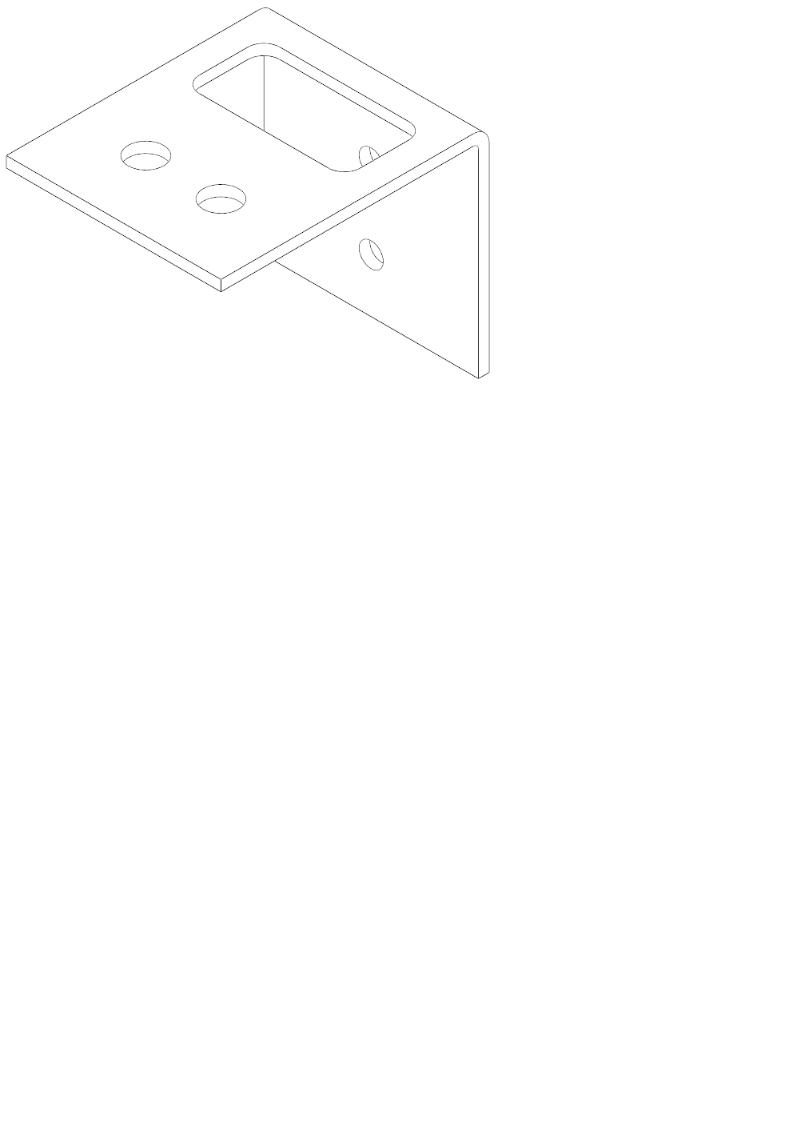
\includegraphics[width = 0.4\textwidth]{assets/figures/SupportChaineCable.png}
  \caption{Représentation du support pour la chaîne porte-câbles}
  \label{fig:SupChaineCable}
\end{figure}

\section{Plaque de passage pour moteur}\label{sec:PlaPassMot}
Afin de cacher un peu plus l'arrière du système pour le rendre présentable et aussi afin d'augmenter la rigidité du système, une plaque est placée
entre les deux profilés centraux. Les pièces faisant la liaison entre le moteur et le glider, décritent dans le chapitre \ref{sec:LiaisonMotGlid},
passent par cet endroit donc il faut découper une zone de passage pour ces pièces. Cela donne la plaque suivante.

\begin{figure}[H]
  \centering
  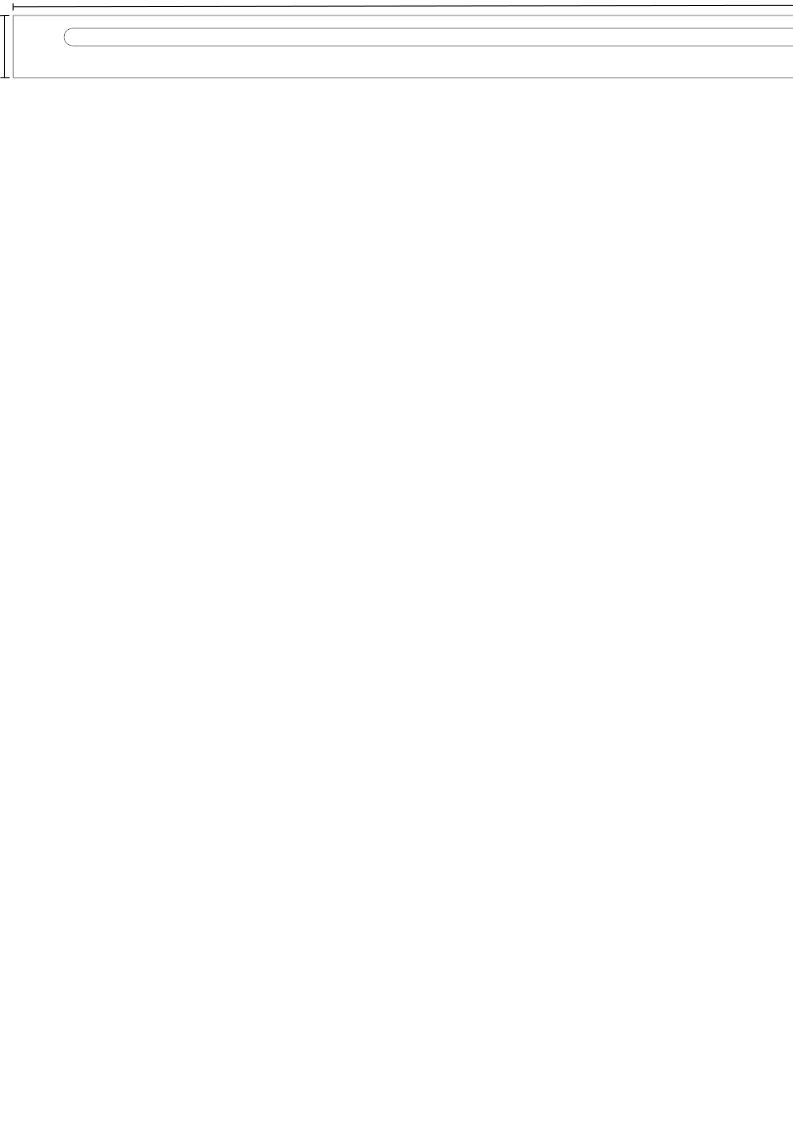
\includegraphics[width = \textwidth]{assets/figures/PlaquePassageMoteur.png}
  \caption{Représentation de la plaque centrale}
  \label{fig:PLaPassMot}
\end{figure}

\section{Assemblage mécanique complet}\label{sec:AssMecComp}
Enfin, voici l'assemblage de toutes les pièces mécaniques fabriquées avec la structure et les composants commandés vu de face et de derrière.

\begin{figure}[H]
  \centering
  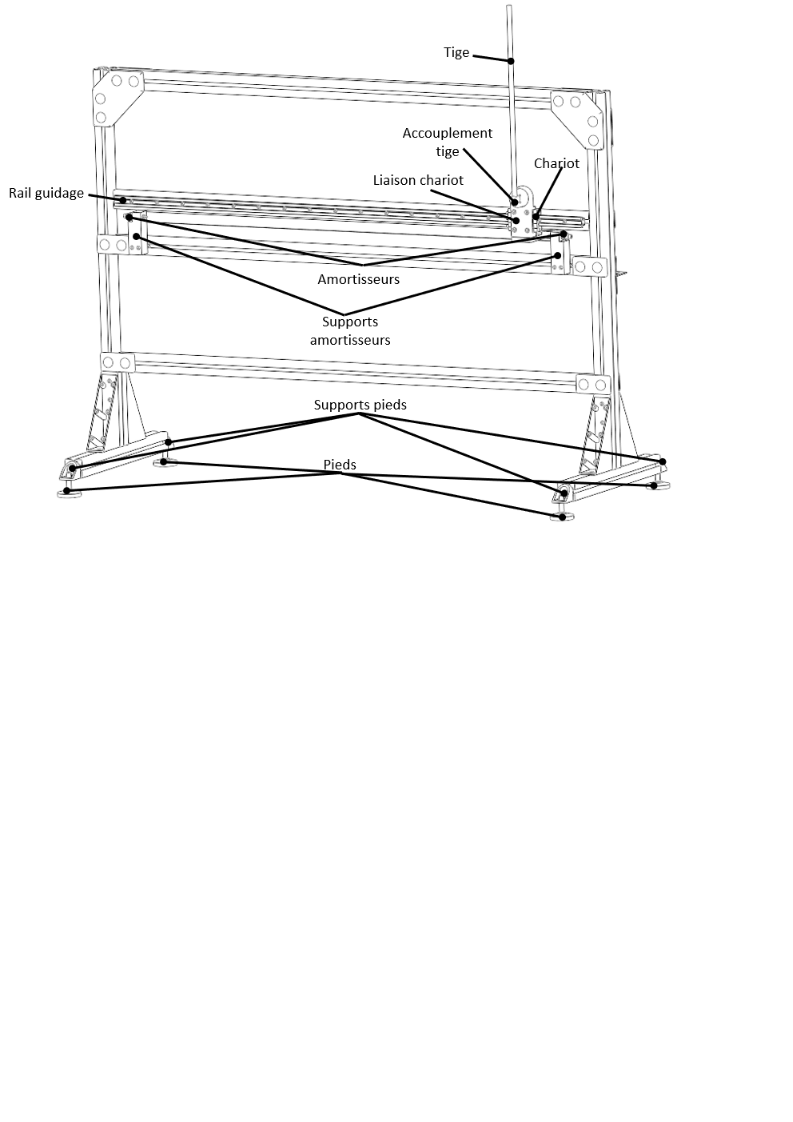
\includegraphics[width = \textwidth]{assets/figures/AssemblageCompletFace.png}
  \caption{Représentation de l'assemblage mécanique complet vu de face}
  \label{fig:AssCompFace}
\end{figure}

\begin{figure}[H]
  \centering
  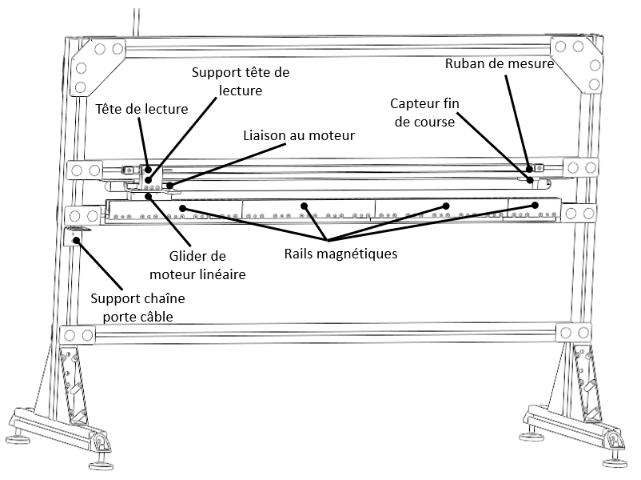
\includegraphics[width = \textwidth]{assets/figures/AssemblageCompletDerriere.png}
  \caption{Représentation de l'assemblage mécanique complet vu de derrière}
  \label{fig:AssCompDerriere}
\end{figure}

\chapter{Boîtier électrique}
\section{Description des connections}\label{sec:DescConnect}
L'ensemble des étages d'alimentation et de commande sont placés dans un boîtier électrique qui se branche sur une prise classique 230~V. Ce dernier
devra alimenter le contrôleur EPOS4 Compact 50/15 de chez Maxon \cite{Maxon} et la carte Raspberry Pi \cite{RaspberryPi}. Une tension continue de 48~V
sera nécessaire pour commander le moteur et une tension continue de 5~V aussi pour alimenter le Raspberry Pi et comme tension logique 1. Pour obtenir
ces tensions, un convertisseur AC-DC avec 48~V en sortie et un convertisseur DC-DC avec 48~V en entrée et 5~V en sortie seront nécessaire. La fiche 230~V
sera une fiche pour appareil C14 avec bouton et fusible intégré ce qui enlève la nécessité de mettre un disjoncteur et fait gagner de la place. Les deux
convertisseurs, le contrôleur et la carte de commande sont tous fixés sur un rail DIN35. Il faut donc déterminer les dimensions de ces éléments pour
déterminer la taille du boîtier et du rail nécessaire.\\

Le contrôleur est aussi connecté à l'encodeur linéaire et angulaire, à l'anneau de LEDs et aux capteurs de fin de course. On peut résumer toutes
ces connections sur le schéma suivant.

\begin{figure}[H]
  \centering
  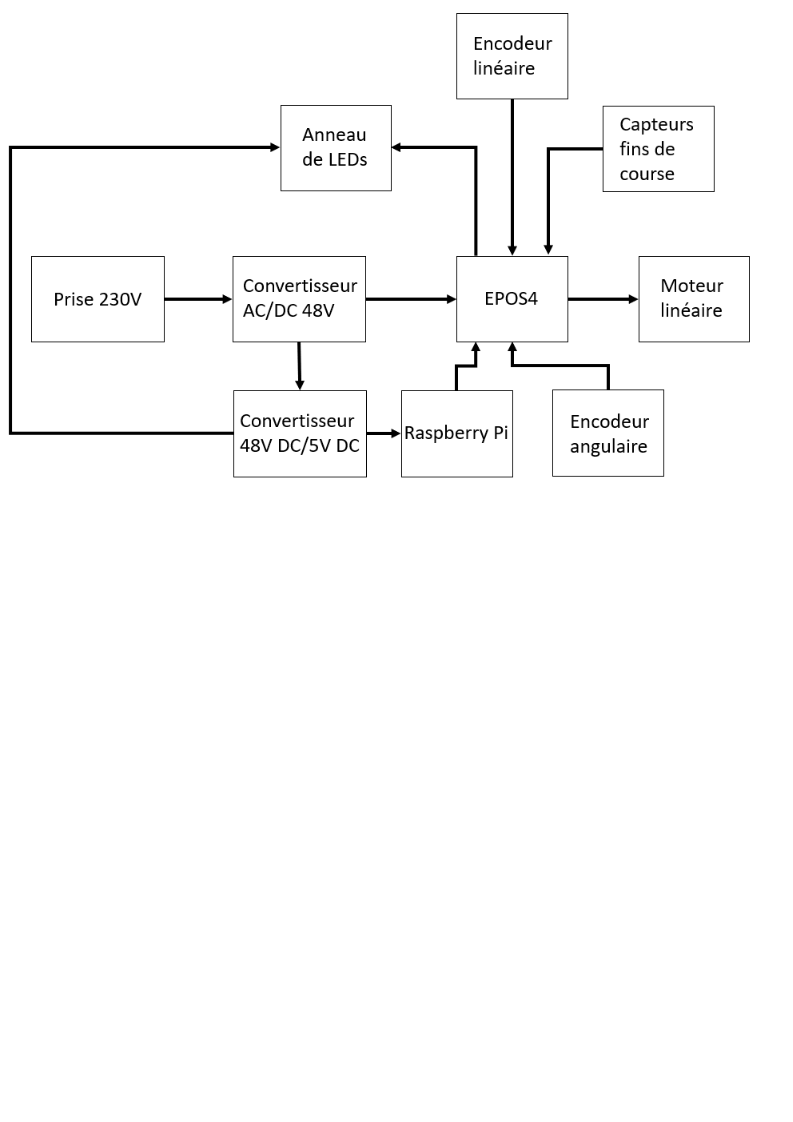
\includegraphics[width = 0.9\textwidth]{assets/figures/SchemaLogique.png}
  \caption{Schéma de connections}
  \label{fig:SchemaConnec}
\end{figure}

\section{Choix des éléments}\label{sec:ChoixElem}

\begin{table}[H]
  \centering
  \caption{Éléments choisis pour le boîtier électrique}
  \label{tab:ChoixElem}
  \resizebox{\textwidth}{!}{%
    \begin{tabular}{|l|l|l|l|l|l|}
      \hline
      Élément                    & Choix               & Fabricant                       & Hauteur {[}mm{]} & Largeur {[}mm{]} & Profondeur {[}mm{]} \\ \hline
      Convertisseur AC-DC 48V    & DRC100US48          & XP Power \cite{XPPower}         & 93               & 70               & 58                  \\ \hline
      Convertisseur DC-DC 48V-5V & DDR-15L-5           & MEAN WELL \cite{MEANWELL}       & 90               & 17.5             & 54.5                \\ \hline
      Contrôleur moteur          & EPOS4 Compact 50/15 & Maxon \cite{Maxon}              & 65.5             & 59.5             & 35                  \\ \hline
      Carte de commande          & Raspberry Pi 4      & Raspberry Pi \cite{RaspberryPi} & 85               & 56               & 30                  \\ \hline
      Connecteur fiche 230V      & C14                 & Schurter \cite{Schurter}        & -                & -                & -                   \\ \hline
      Bouton arrêt d'urgence     & AB6E-3BV02PTRH      & IDEC \cite{IDEC}                & -                & -                & -                   \\ \hline
      Bouton poussoir            & 82-5151.1134.B001   & EAO \cite{EAO}                  & -                & -                & -                   \\ \hline
    \end{tabular}%
  }
\end{table}

La somme des largeurs des éléments est de 203~mm, la hauteur la plus grande est de 93~mm et la profondeur la plus élevée est de 58~mm. Le choix
du boîtier se porte sur l'ABS 200/100 HG ENCLOSURE de chez Fibox \cite{Fibox} avec 171~mm de hauteur interne, 95~mm de profondeur interne et
246~mm de largeur interne. Avec il y aussi la plaque de montage MIV 200 MOUNTING PLATE et le rail MIV 20 DIN-35 RAIL aussi de chez Fibox \cite{Fibox}.
Les connections entre les éléments externes et internes au boîtier doivent être faites de manière à ce qu l'on puisse déconnecter les éléments
externes et retirer le boîtier sans avoir à démonter le reste du système. À cette fin, plusieurs connecteurs sont utilisés pour faire l'interface
entre l'intérieur et l'extérieur du boîtier et, pour les éléments ne possédant que 2 ou 3 fils minces qui ne nécessitent pas un connecteur
individuel, des presses étoupes sont utilisés comme passage de câbles. Ces câbles là viennent se fixer sur un bornier de 25~mm de large situé
sur le rail DIN35. L'ajout d'un bornier sur le rail prend cependant trop de place avec la configuration actuelle des autres composants, c'est
donc pour cela que la décision de venir fixer la carte RaspberryPi sur son côté a été prise. Ainsi, la place gagnée en changeant la position du
RaspberryPi est de 26~mm et la place utilisée par le bornier est de 25~mm. L'espace dans le boîtier est donc toujours suffisant.
L'assemblage de ces pièces ressemble à ceci.

\begin{figure}[H]
  \centering
  \includegraphics[width = 0.8\textwidth]{assets/figures/AssemblageBoitierElectrique.png}
  \caption{Boîtier électrique avec composants}
  \label{fig:AssBoitierElec}
\end{figure}

\chapter{Liste de matériel}
\section{Matériel acheté}\label{sec:MatAchete}

\begin{table}[H]
  \centering
  \caption{Liste de pièces achetées}
  \label{tab:ListeAchete}
  \resizebox{\textwidth}{!}{%
    \begin{tabular}{|l|l|l|l|l|}
      \hline
      \textbf{Élément}            & \textbf{Nom}                     & \textbf{Fabricant}              & \textbf{Prix [CHF]}        & \textbf{Quantité} \\ \hline
      Profilé                     & Profilé 8 40x40x1120             & Item \cite{Item}                & 47                         & 4                 \\ \hline
      Profilé                     & Profilé 8 40x40x800              & Item \cite{Item}                & 47                         & 2                 \\ \hline
      Profilé                     & Profilé 8 40x40x400              & Item \cite{Item}                & 37                         & 2                 \\ \hline
      Plaques                     & Plaques automatique 8 120x120    & Item \cite{Item}                & 23                         & 4                 \\ \hline
      Plaques                     & Plaques automatique 8 80x40      & Item \cite{Item}                & 11                         & 10                \\ \hline
      Equerres                    & Kit équerre 8 160x80             & Item \cite{Item}                & 29                         & 4                 \\ \hline
      Ecrous                      & Ecrou 8 Zn M4                    & Item \cite{Item}                & 2                          & 12                \\ \hline
      Ecrous                      & Ecrou 8 Zn M3                    & Item \cite{Item}                & 2                          & 17                \\ \hline
      Profilé                     & Profilé en U 8 rouge             & Item \cite{Item}                & 6                          & 10                \\ \hline
      Embouts                     & Embout 8 40x40 noir              & Item \cite{Item}                & 1                          & 2                 \\ \hline
      Pieds                       & GN 6311.6-50-M10-37-KR           & Elesa \cite{Elesa}              & 39                         & 4                 \\ \hline
      Moteur                      & AUM2-S3                          & TDS \cite{TDSPrecisionProducts} & 1020                       & 1                 \\ \hline
      Fin de course               & MC-38                            & Synacorp \cite{Synacorp}        & 2                          & (2)               \\ \hline
      Amortisseur                 & RB1007                           & SMC \cite{SMC}                  & 64                         & 2                 \\ \hline
      Chariot                     & WW-10-30-T15-AL-J200             & Igus \cite{Igus}                & 64                         & 1                 \\ \hline
      Rail                        & WS-10-30 1100~mm                 & Igus \cite{Igus}                & 62                         & 1                 \\ \hline
      Chaîne porte câble          & System E2 mini Series 14 1220~mm & Igus \cite{Igus}                & 34                         & 1                 \\ \hline
      Ruban de mesure             & LIDA405 840~mm                   & Heidenhain \cite{Heidenhain}    & -                          & (1)               \\ \hline
      Tête de lecture             & LIDA48                           & Heidenhain \cite{Heidenhain}    & -                          & (1)               \\ \hline
      Support ruban               & 311131-09                        & Heidenhain \cite{Heidenhain}    & 177                        & 1                 \\ \hline
      Encodeur                    & TMCS-20                          & Trinamic \cite{Trinamic}        & 90                         & (1)               \\ \hline
      Roulement                   & SKF W 61700 X-2RS1               & SKF \cite{SKF}                  & -                          & 2                 \\ \hline
      Anneau de LEDs              & NeoPixel Ring 12x RGBW LEDs      & Adafruit \cite{Adafruit}        & 10                         & 1                 \\ \hline
      Boîtier électrique          & ABS 200/100 HG                   & Fibox \cite{Fibox}              & 51                         & 1                 \\ \hline
      Rail DIN                    & MIV 20 DIN-35 255~mm             & Fibox \cite{Fibox}              & 6                          & 1                 \\ \hline
      Plaque de montage           & MIV 200                          & Fibox \cite{Fibox}              & 7                          & 1                 \\ \hline
      Convertisseur DC/DC         & DDR-15L-5                        & MEAN WELL \cite{MEANWELL}       & 29                         & 1                 \\ \hline
      Convertisseur AC/DC         & DRC100US48                       & XP Power \cite{XPPower}         & 41                         & 1                 \\ \hline
      Fiche 230V                  & C14                              & Schurter \cite{Schurter}        & 16                         & 1                 \\ \hline
      Arrêt d'urgence             & AB6E-3BV02PTRH                   & IDEC \cite{IDEC}                & 46                         & 2                 \\ \hline
      Bouton                      & 82-5151.1134.B001                & EAO \cite{EAO}                  & 35                         & 1                 \\ \hline
      Contrôleur moteur           & EPOS4 Compact 50/15              & Maxon \cite{Maxon}              & 660                        & (1)               \\ \hline
      Carte microcontrôleur       & Raspberry Pi 4                   & Raspberry Pi \cite{RaspberryPi} & -                          & (1)               \\ \hline
      Module de communication CAN & RS485 CAN HAT                    & Waveshare \cite{Waveshare}      & 21                         & 1                 \\ \hline
      \textbf{Total dépensé}      & -                                & -                               & \textbf{2783}\footnotemark & -                 \\ \hline
    \end{tabular}%
  }
\end{table}

\footnotetext{Les quantités entre parenthèses indiquent que l'objet n'a pas été acheté car déjà dans l'inventaire de l'école. Le coût de ces objets n'est pas pris en compte dans ce total.}

\section{Matériel fabriqué}\label{sec:MatFab}

\begin{table}[H]
  \centering
  \caption{Liste de pièces fabriquées}
  \label{tab:ListeFab}
  \resizebox{\textwidth}{!}{%
    \begin{tabular}{|l|l|l|l|}
      \hline
      \textbf{Pièce}             & \textbf{Matière} & \textbf{Dimensions} & \textbf{Quantité} \\ \hline
      Support pied               & EN-AW 6082       & 40x40x40            & 4                 \\ \hline
      Support chaîne porte câble & EN-AW 5052       & 40x40x50            & 1                 \\ \hline
      Support amortisseur        & EN-AW 6082       & 28x30x90            & 2                 \\ \hline
      Liaison moteur             & EN-AW 6082       & 100x123x15          & 1                 \\ \hline
      Liaison chariot            & EN-AW 6082       & 108.5x46x25         & 1                 \\ \hline
      Support tête de lecture    & EN-AW 6082       & 46x51x25            & 1                 \\ \hline
      Accouplement encodeur      & EN-AW 6082       & $\emptyset$24x32    & 1                 \\ \hline
      Accouplement tige          & \acrshort{PMMA}  & $\emptyset$38x42    & 1                 \\ \hline
      Tige                       & \acrshort{PMMA}  & $\emptyset$10x420   & 1                 \\ \hline
      Plaque passage moteur      & EN-AW 6060       & 80x4x1135           & 1                 \\ \hline
      Plaque assemblage 1        & EN-AW 6082       & 32x2x119            & 1                 \\ \hline
      Plaque assemblage 2        & EN-AW 6082       & 32x2x299            & 3                 \\ \hline
    \end{tabular}%
  }
\end{table}

\chapter{Conclusion}
Lors de ce projet, différentes parties du pendule inversé ont été réalisées. Tout d'abord, la mécanique du système incluant le guidage, la motorisation
et la mise en place de capteurs a été faîte en suivant les demandes posées en début de projet. Ensuite, la partie électrique avec l'alimentation du
système et sa commande a aussi été développée pendant ce temps. Une grande quantité de pièces ont été commandées chez différents fabricants pour
pouvoir construire ce projet. Ceci a requis du temps pour trouver et négocier des offres avec un prix et des temps de livraisons raisonnables
pour rester dans le cadre du travail de Bachelor. D'autres pièces ont été développées personnellement et seront fabriquées par l'école.\\

Les étapes restantes à effectuer pendant la seconde partie du \acrshort{TB} sont: l'assemblage de tous les éléments commandés pour avoir un
système fonctionnel, la programmation de la commande \gls{PID} et les tests sur le fonctionnement du système.

\chapter*{Remerciements}
Je tiens à adresser ces remerciements aux personnes qui m'ont aidé lors de ce projet.\\

Merci à Monsieur Yves Chevallier pour avoir suivi et aidé tout le long du projet.
\newline
Merci à Monsieur Mikaël Krummen pour son aide sur la création et la mise en plan de pièces mécaniques.
\newline
Merci à Monsieur Pierre-François Gauthey pour son aide et ses suggestions pour les pieds réglables et supports du système.
\newline
Merci à Monsieur Marc-André Bovet pour son aide avec les commandes de matériel et les discussions avec les fournisseurs.
\newline
Et merci à toutes les personnes de ma classe et les personnes présentes en C26 pour leur aide et leur support tout le long du projet.

\clearpage
\printbibliography

\appendix
\appendixpage
\addappheadtotoc

\section*{Annexes}
\addcontentsline{toc}{section}{Annexes}
\subsubsection*{Planning de projet}
\subsubsection*{Fiches techniques}

%Anneau de LEDs
\textbf{Anneau de LEDs Adafruit NeoPixel Ring, Berrybase}

% Boitier et composants d'alimentation
\textbf{Boitier MNX ABS 200/100 HG, FIBOX}
\newline \textbf{Arrêt d'urgence X6 Series, IDEC}
\newline \textbf{Bouton d'alimentation C14 250V, Schurter}
\newline \textbf{Bouton lumineux 19mm, eao}
\newline \textbf{Convertisseur AC-DC 48V TBLC50, Traco Power}
\newline \textbf{Convertisseur 48V-5V DDR-15L-5, MEAN WELL}

% Encodeur
\textbf{Encodeur TMCS-20, Trinamic}
\newline
\textbf{Montage encodeur TMCS-20, Trinamic}

% Roulements
\textbf{Roulement 61700 X-2RS1, SKF}

% Moteur linéaire
\textbf{Moteur linéaire AUM2-S3, TDS}

% Driver Moteur
\textbf{Driver moteur EPOS4 Compact 50/15, Maxon}

% Règle linéaire
\textbf{Règle linéaire LIDA 405, Heidenhain}
\newline
\textbf{Tête de lecture LIDA 405, Heidenhain}

% Pieds réglables
\textbf{Pieds réglables GN6311.6, Elesa}

%Mises en plans des pièces mécaniques
\textbf{Mise en plan du couplage de l'encodeur}
\newline \textbf{Mise en plan du couplage de la tige}
\newline \textbf{Mise en plan de la liaison du chariot}
\newline \textbf{Mise en plan de la liaison du moteur}
\newline \textbf{Mise en plan du support de l'amortisseur}
\newline \textbf{Mise en plan du deuxième support de l'amortisseur}
\newline \textbf{Mise en plan du support de guidage de câble}
\newline \textbf{Mise en plan du support des pieds}
\newline \textbf{Mise en plan du support de la tête de lecture}

\iffalse

  %Anneau de LEDs
  \includepdf[pages=-]{Annexes/anneau de Led.pdf}

  % Boitier et composants d'alimentation
  \includepdf[pages=-]{Annexes/Boitier alimentation}
  \includepdf[pages=-]{Annexes/Arret d'urgence}
  \includepdf[pages=-]{Annexes/Bouton d'alimentation}
  \includepdf[pages=-]{Annexes/Bouton lumineux}
  \includepdf[pages=-]{Annexes/Convertisseur AC-DC 48V}
  \includepdf[pages=-]{Annexes/Convertisseur 48V-5V}

  % Encodeur
  \includepdf[pages=-]{Annexes/Encodeur TMCS-20}
  \includepdf[pages=-]{Annexes/Montage encodeur}

  % Roulements
  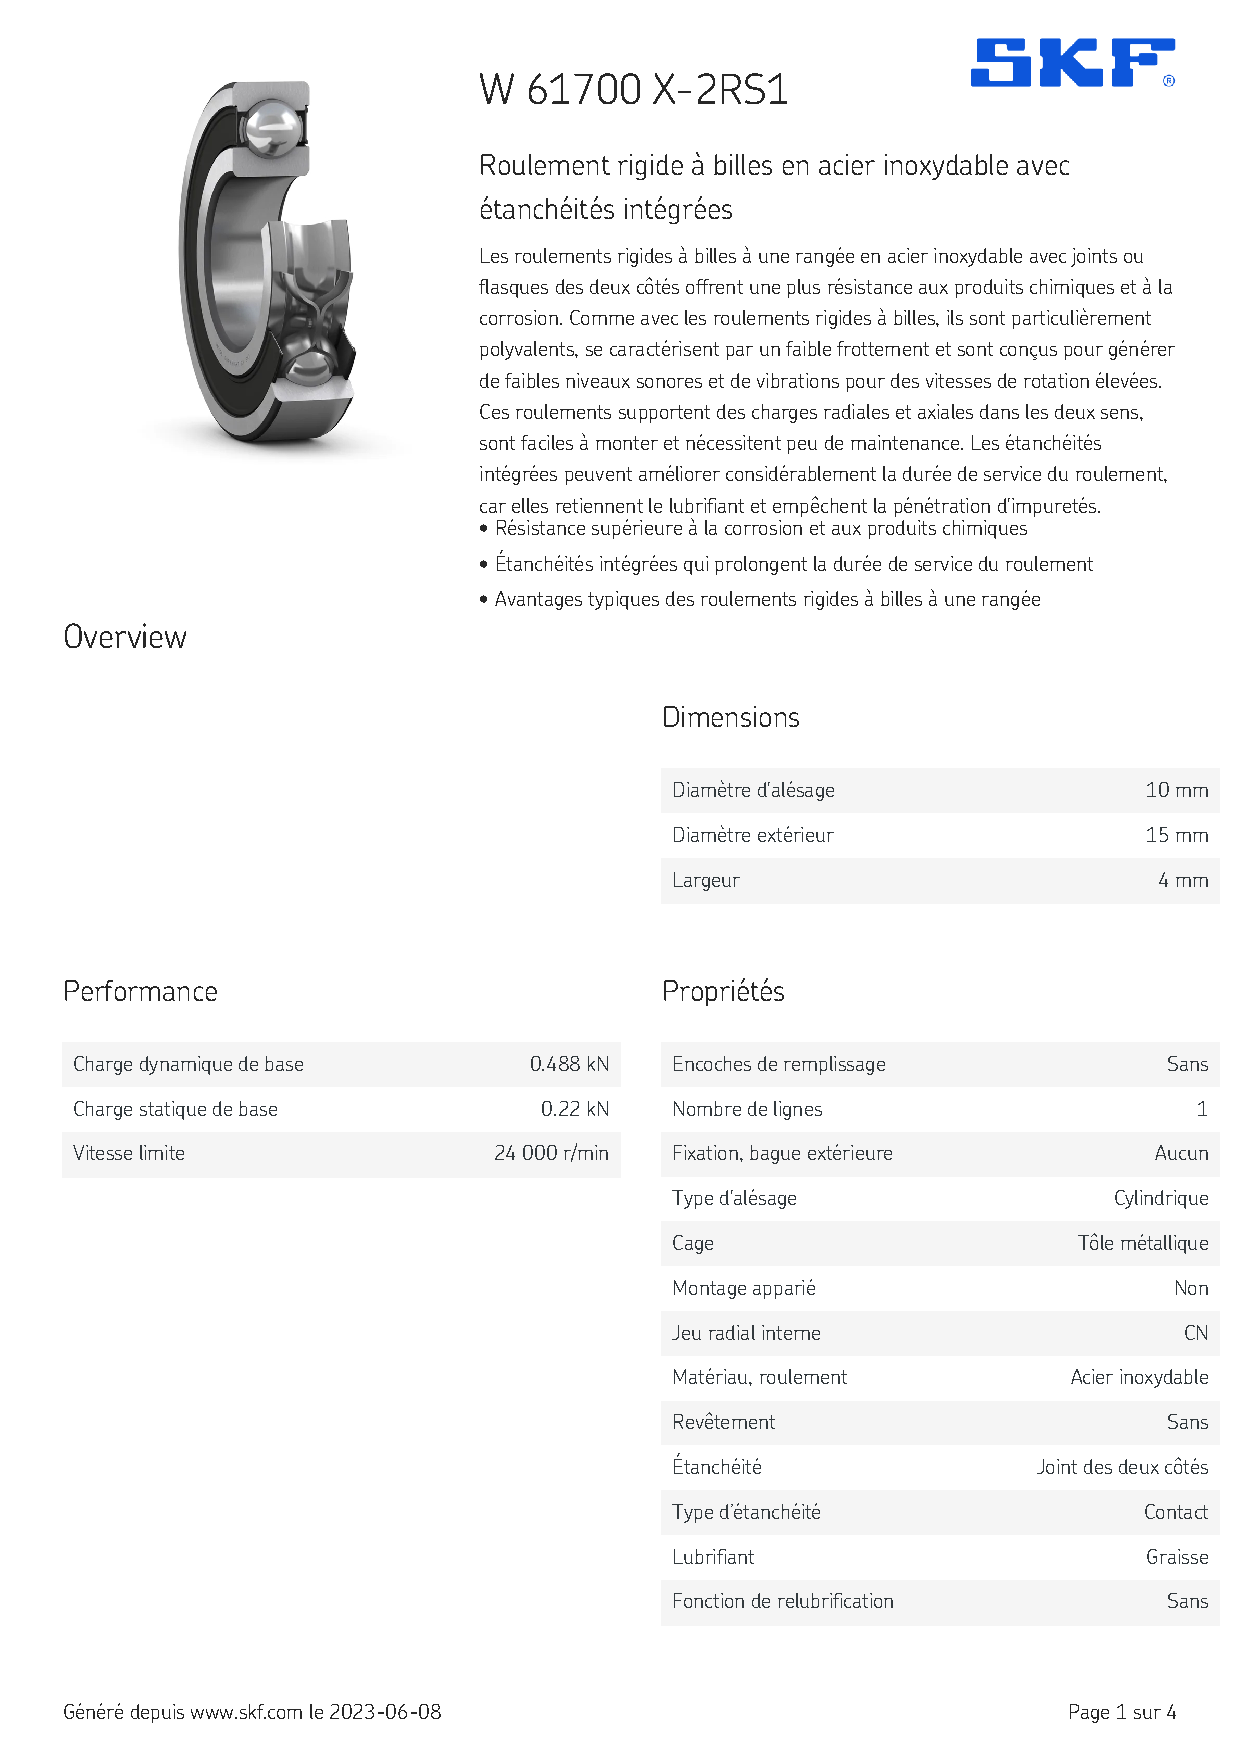
\includepdf[pages=-]{Annexes/Roulement SKF W 61700 X-2RS1}

  % Moteur linéaire
  \includepdf[pages=-]{Annexes/Moteur lineaire}

  % Driver Moteur
  \includepdf[pages=-]{Annexes/EPOS4-Module-Compact}

  % Règle linéaire
  \includepdf[pages=-]{Annexes/Montage regle lineaire}
  \includepdf[pages=-]{Annexes/Tete de lecture}

  % Pieds réglables
  \includepdf[pages=-]{Annexes/Pieds reglable}

  %Mises en plans des pièces mécaniques
  \includepdf[pages=-]{Annexes/MEP Couplage Encodeur}
  \includepdf[pages=-]{Annexes/MEP Couplage Tige}
  \includepdf[pages=-]{Annexes/MEP Liaison chariot}
  \includepdf[pages=-]{Annexes/MEP Liaison Moteur}
  \includepdf[pages=-]{Annexes/MEP Support Amortisseur}
  \includepdf[pages=-]{Annexes/MEP Support Amortisseur 2}
  \includepdf[pages=-]{Annexes/MEP Support Guidage Cable}
  \includepdf[pages=-]{Annexes/MEP Support Pieds}
  \includepdf[pages=-]{Annexes/MEP Support Tete Lecture}

\fi

\let\cleardoublepage\clearpage
\backmatter

\label{glossaire}
\printnoidxglossary
\label{index}
\printindex

% Le colophon est le dernier élément d'un document qui contient des notes de l'auteur concernant la mise en page et l'édition du document : il est parfaitement optionnel.
\input{colophon.tex}

\end{document}
